\documentclass{article}

% Recommended ICML packages.
\usepackage{microtype}
\usepackage{graphicx}
\usepackage{subcaption}
\usepackage{booktabs}
\usepackage{hyperref}
\usepackage{amsmath}
\usepackage{amssymb}
\usepackage{mathtools}
\usepackage{placeins}
\usepackage{float}
\usepackage{etoolbox}
\usepackage{xcolor}
\usepackage{pgffor}
\usepackage{hyperref}
\usepackage[capitalize,noabbrev]{cleveref}
\crefname{appendix}{Appendix}{Appendices}
\Crefname{appendix}{Appendix}{Appendices}

\input{commenting}

% Blind workshop submission. If accepted, switch to:
% \usepackage[accepted]{icml2026}
\usepackage{icml2026}

% Local notation. Keep custom macros minimal and do not use them in the title.
\newcommand{\zscore}{\ensuremath{z = (x-\mu)/\sigma}}
\newcommand{\primalz}{\ensuremath{d_{z}}}
\newcommand{\primalx}{\ensuremath{d_{x}}}
\newcommand{\logitdiff}{\ensuremath{\Delta_{\mathrm{logit}}}}
\newcommand{\redtodo}[1]{\textcolor{red}{\textbf{[TODO]} #1}}

\icmltitlerunning{The Geometry of Relativity}

\begin{document}

\twocolumn[
  \icmltitle{The Geometry of Relativity: Context-Relative Scalar Representations in LLMs}

  % The style file suppresses author information in the blind version.
  \begin{icmlauthorlist}
    \icmlauthor{Anonymous Authors}{anon}
  \end{icmlauthorlist}

  \icmlaffiliation{anon}{Anonymous Institution}
  \icmlcorrespondingauthor{Anonymous Authors}{anonymous@example.com}
  \icmlkeywords{mechanistic interpretability, representation geometry, language models, gradable adjectives}

  \vskip 0.3in
]

% Required by the ICML style, even for anonymous submissions.
\printAffiliationsAndNotice{}


\begin{abstract}
Human judgments of gradable adjectives, such as \emph{tall} and \emph{short}, are fundamentally context-dependent, relying on relative standing rather than absolute values. In this paper, we investigate whether large language models exhibit similar context-sensitive reasoning, mirroring human cognitive patterns. We first show behaviorally that when given in-context examples defining a comparison class, model predictions are governed primarily by context-normalized standing rather than raw magnitude. This behavior emerges with even a single reference value, becomes smoother
with richer comparison classes, and shows human-like sensitivity to presentation order and distribution shape, including recency and local-cluster effects. We then analyze the model's internal representations and find that this context-normalized standing is linearly decodable from model activations. Furthermore, through causal steering, shared-direction transfer, and attention-based interventions, we show that this context-relative representation is functionally utilized by the model and partially shared across diverse semantic domains. Together, our results suggest that LLMs construct a context-relative scalar representation that is behaviorally dominant, internally accessible, and causally relevant.
\end{abstract}

\section{Introduction}
\label{sec:introduction}

Gradable adjectives such as \emph{tall} and \emph{short} are context-dependent. In everyday language, we often rely on broad world knowledge when applying them: a person who is 175 cm tall might be described as tall in general conversation.
However, this judgment can shift dramatically when a comparison class is made explicit.
Among professional basketball players, the same individual would likely be considered short, as illustrated in \Cref{fig:setup-pipeline}.

This flexibility suggests that human judgments are not based solely on absolute values, but instead depend on a relative standing within a context. The main question of this paper is whether large language models (LLMs) exhibit a similar form of context-sensitive reasoning. When given in-context examples that implicitly define a comparison class, do LLMs base their predictions on raw numerical values or relative standings? Moreover, beyond behavioral observations, we investigate the underlying mechanisms: how do the internal representations of LLMs encode these contexts to ultimately drive the selection of a specific adjective?

\begin{figure}[t]
  \centering
  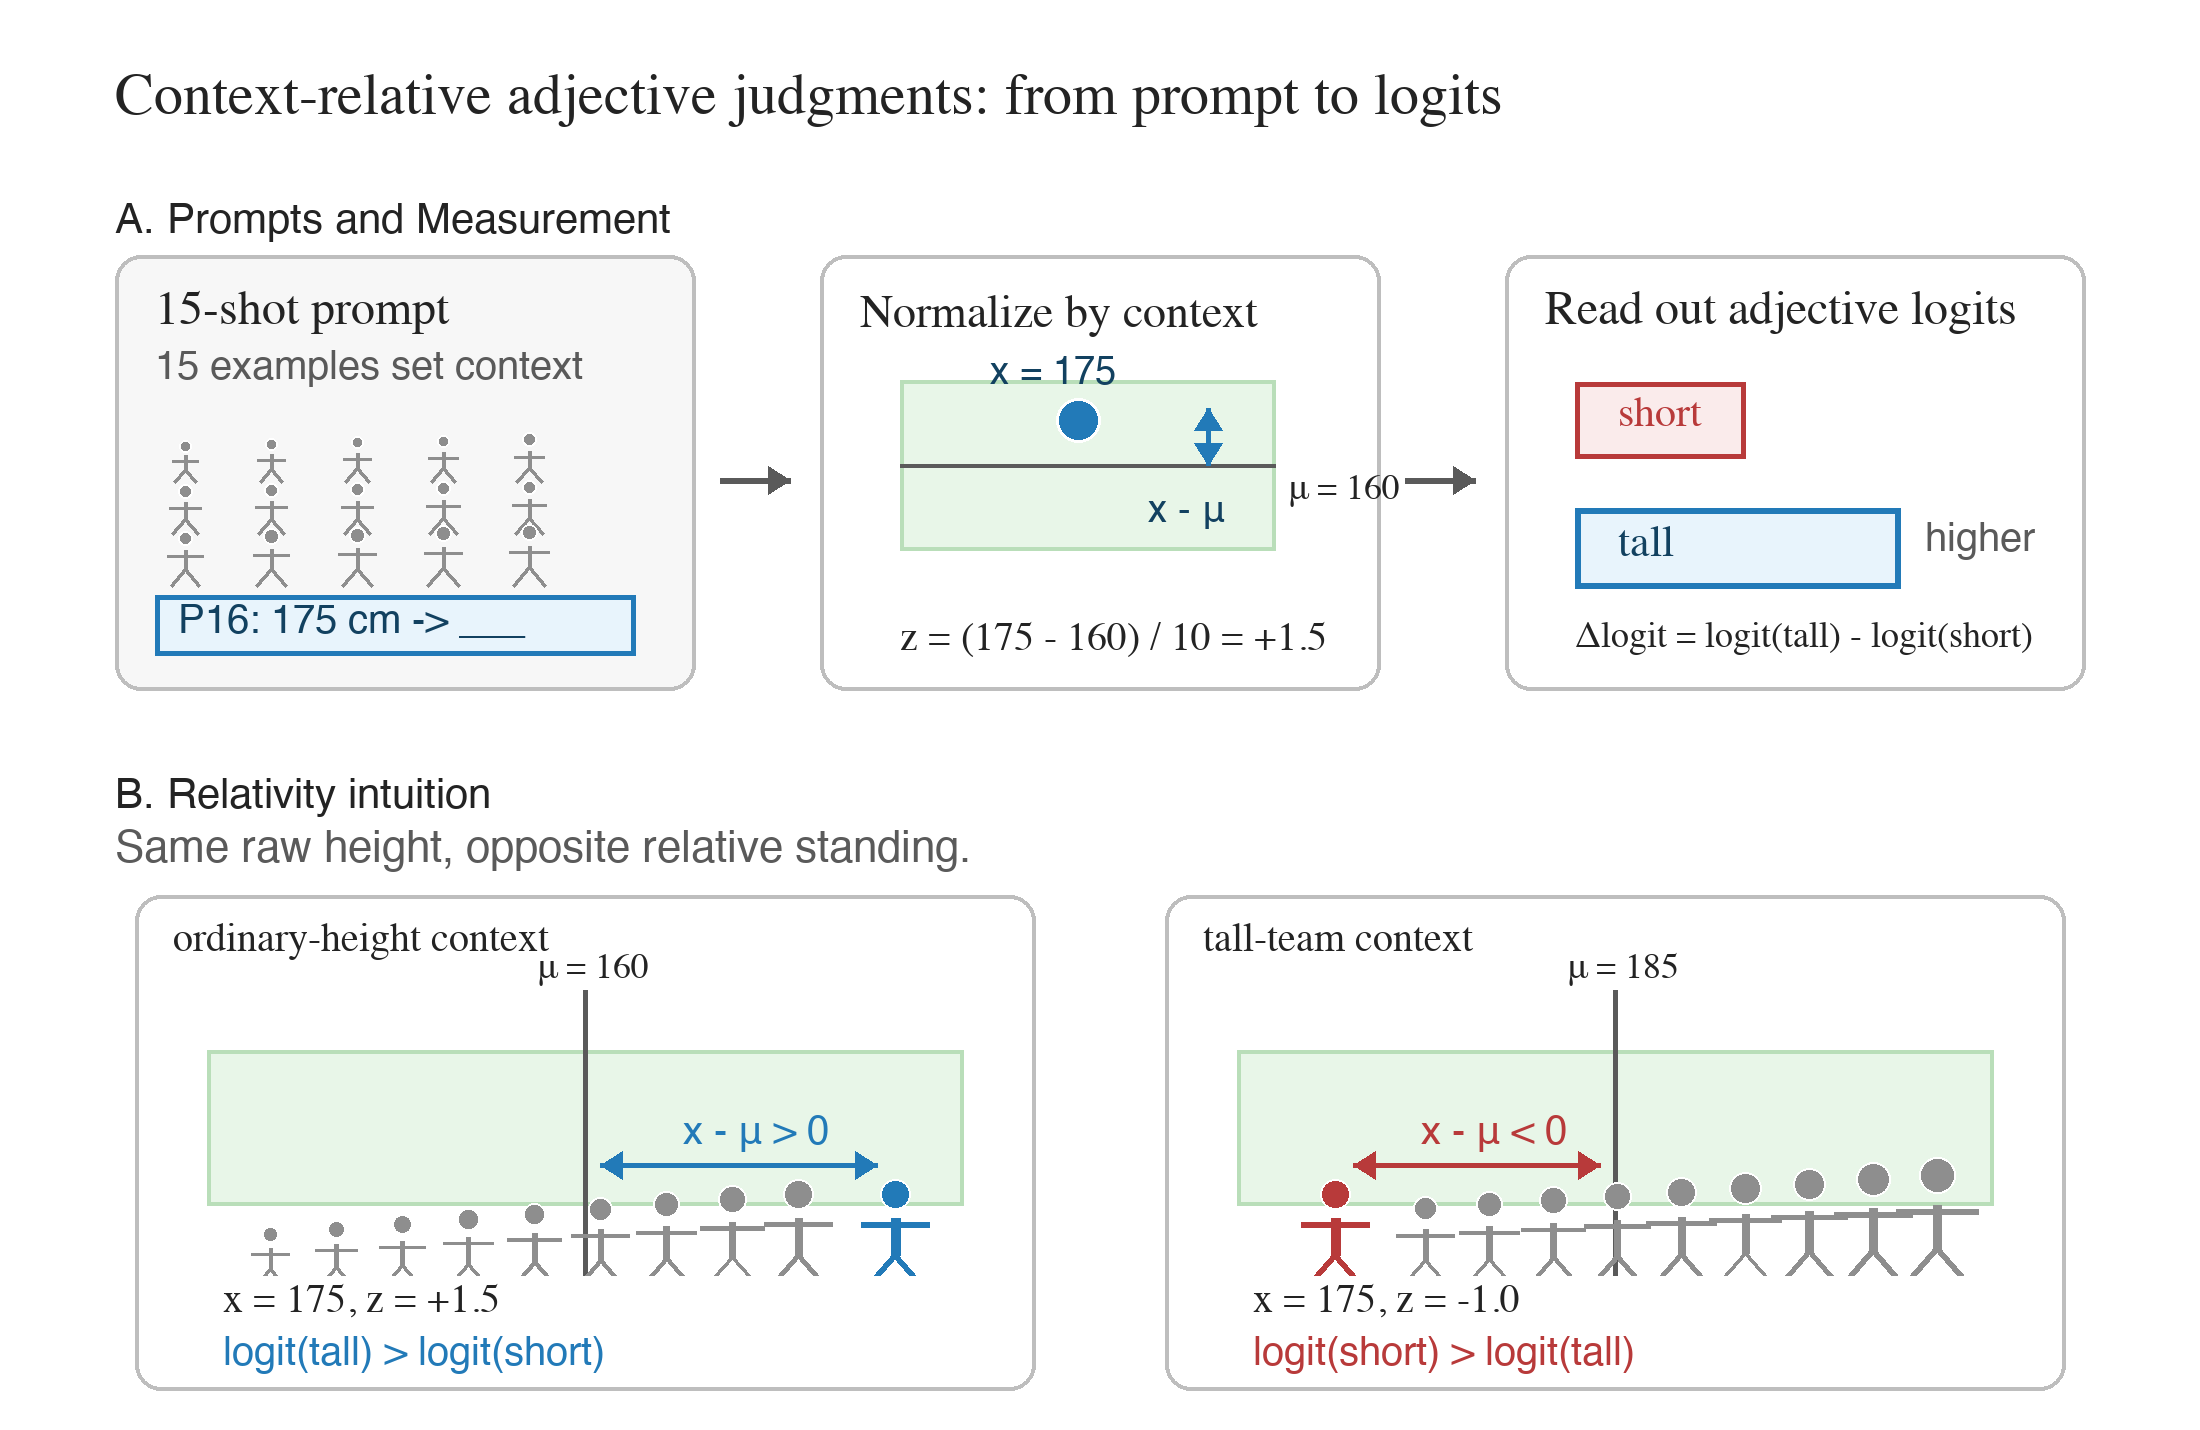
\includegraphics[width=\linewidth, trim={100 10 100 150}, clip]{figures/candidates_png/candidate_5_combined_pipeline_relcontrast.png}
  \caption{\textbf{Prompt and measurement schematic.}
  Context examples define a local comparison class.
  We compute the target's normalized standing and measure whether the model assigns a higher logit to the high adjective or the low adjective.
  }
  \label{fig:setup-pipeline}
\end{figure}


To investigate this, we adopt a mechanistic interpretability perspective grounded in the linear representation hypothesis \citep{park2024linear}. While prior work has established that LLM activations linearly encode absolute high-level concepts \citep{marks2023geometry,arditi2024refusal}, capturing context-dependent relationships requires viewing these features as higher-dimensional abstractions \citep{gurnee2026manifold,modellerubin2025manifolds}. By leveraging these geometric frameworks and manifold steering interventions \citep{sarfati2026beliefs, park2026softmaxgeometry}, we can isolate how comparative judgments are represented and manipulated within the model's layers.

To that end, our contributions are as follows:
\begin{itemize}
    \item We empirically show that gradable adjective judgments in LLMs are primarily governed by a context-normalized standing of in-context examples rather than raw magnitude. Moreover, we show that these behaviors are affected by the number, order, and distribution of the reference values.
    
    \item We demonstrate that this context-normalized standing is linearly decodable, and that its direction can be causally used to predict high-minus-low adjective logit differences across diverse semantic domains and models.

    \item We provide causal evidence via steering and attention-based interventions that this relativistic representation is functionally used by the model and is partially shared across adjective concepts, rather than being purely concept-specific.
\end{itemize}

\section{Experiment Design}
\label{sec:experiment_design}
We use Gemma-2-9B \citep{gemma2_2024} and focus on eight adjective pairs, as shown in \Cref{tab:domains}.
Our goal is to understand how LLMs process a given raw value---e.g., 170 cm---when other values are previously given.
We seek to understand whether LLMs would use the raw value $x$ directly, or a context-normalized standing:
\begin{align*}
    z = \frac{x-\mu}{\sigma},
\end{align*}
where $\mu$ is a context mean (the average of the reference values) and $\sigma$ is a context spread (the standard deviation of the reference values).
We refer to models that use only $x$ as \emph{objective} and models that use $z$ as \emph{relativistic}.





\begin{table}[t]
  \centering
  \footnotesize
  \setlength{\tabcolsep}{3pt}
  \caption{\textbf{Adjective-pair prompt domains.}
  The dense prompt grid samples target values $x$ over the listed ranges, in the listed units, and uses the shown context spread $\sigma$.
  Income is used as the measured proxy for wealth; its normalization is log-space, so $\sigma=\log 2$ means one unit of normalized spread corresponds to doubling or halving annual income.}
  \label{tab:domains}
  \resizebox{\columnwidth}{!}{%
  \begin{tabular}{lllll}
    \toprule
    Concept & Unit & Low/High & $\sigma$ & $x$ range \\
    \midrule
    Height & cm & short/tall & 10 & 147--183 \\
    Age & yr & young/old & 5 & 16--64 \\
    Weight & kg & light/heavy & 8 & 45--105 \\
    Size & cm diameter & small/big & 6 & 0.5--65.5 \\
    Speed & km/h & slow/fast & 15 & 7--163 \\
    Income & $\log(\mathrm{USD/yr})$ & poor/rich & $\log 2$ & \$14k--\$900k \\
    Experience & years & novice/expert & 4 & 0.5--27.4 \\
    BMI & kg/m$^2$ & thin/obese & 3 & 14.9--40.1 \\
    \bottomrule
  \end{tabular}}
\end{table}

\subsection{Prompts}
\label{subsec:prompts}
To generate prompts for an adjective pair in \Cref{tab:domains}, we first independently sample the raw value $x$ and the relative standing $z$ from uniform distributions ($x$ is drawn from its domain-specific range and $z \sim \mathcal{U}(-3, 3)$). We then compute the corresponding context mean $\mu$ using the domain's realistic standard deviation $\sigma$.

Next, we generate $k$ in-context reference values, randomly sampled from a normal distribution:
\begin{align*}
    c_1,\ldots,c_k \overset{i.i.d.}{\sim} \mathcal{N}(\mu,\sigma^2).
\end{align*}
These values are formatted into a context list with one entry per line (e.g.\ ``Person 1: $c_1$~cm''), and the target value is appended as a final entry that stops at the adjective cliff (e.g.\ ``Person $k{+}1$: $x$~cm. This person is''); the entity noun and units follow the domain.

Unless otherwise specified, we use a context length of $k=15$ for most analyses. To thoroughly evaluate the model's relativistic capabilities, we examine its behavior under three varying conditions: (1) modifying the number of reference values $k$, (2) permuting the presentation order of the same context values, and (3) sampling from non-Gaussian context distributions with matched means and variances.


\subsection{Methods}
\label{subsec:methods}
We use several measurement and intervention methods to distinguish behavioral effects, linear decodability, geometry, and causal use of variables in the residual stream.

\paragraph{Logit-based behavioral readout}
For each prompt, we compute the high-minus-low adjective logit difference (LD):
\begin{align*}
    \logitdiff = \mathrm{logit}(\text{high adjective}) -
\mathrm{logit}(\text{low adjective}).
\end{align*}
For example, $\logitdiff=\mathrm{logit}(\text{`tall'})-\mathrm{logit}(\text{`short'})$ for height.
Positive values indicate the model leans toward the high adjective.
This logit difference serves as the primary behavioral signal.

\paragraph{Linear probes}
To test linear decodability of $x$ and $z$, we fit ridge regression probes on residual-stream activations $h_L$ at layer $L$ to each target variable:
\[
\hat y = h_L w + b.
\]
We report cross-validated $R^2$ on held-out prompts.
Probes are trained independently per layer and per adjective pair unless otherwise noted.

\paragraph{Mean-difference directions}
We construct a direction in the activation space by contrasting high and low subsets:
\[
d_{z,L}
= \mathbb{E}[h_L \mid z>1] - \mathbb{E}[h_L \mid z<-1],
\]
with an analogous definition for $d_{x,L}$.
These directions are computed on a training split and reused for steering and transfer experiments.


\paragraph{Linear steering}
To test causal relevance, we intervene on the residual stream at layer $L$ by adding a scaled direction:
\begin{align*}
    h_L \leftarrow h_L \pm \alpha \hat d,
\end{align*}
where $\hat d$ is a unit-normalized direction and $\alpha$ is a scalar.
We measure the resulting change in $\logitdiff$ and report the corresponding steering slope:
\begin{align*}
    \frac{\mathbb{E}[\mathrm{LD}(h+\alpha\hat d)-\mathrm{LD}(h-\alpha\hat d)]}{2\alpha},
\end{align*}
which indicates an intervention effect on the logit difference per unit $\alpha$.


We further use a manifold steering method \citep{sarfati2026beliefs}, and attention-based ablations, which will be explained in \Cref{sec:mechanistic-results}.

\section{Behavioral Results}
\label{sec:results}
We begin by investigating model behaviors when provided with contextual reference values.

\begin{figure}[t]
  \centering
  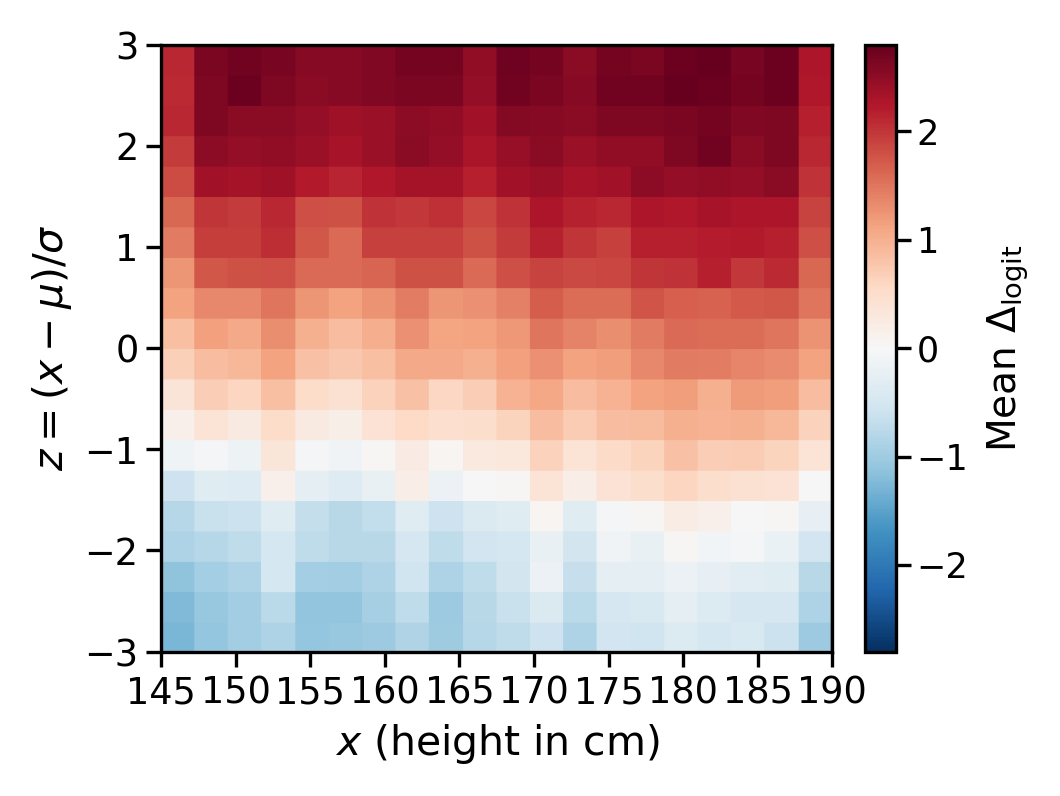
\includegraphics[width=\linewidth]{figures/fig_results_dense_height_heatmap_clean.png}
  \caption{\textbf{Logit differences correlate more strongly with the context-normalized standing $z$ than with the raw value $x$.}
  The heatmap displays the mean logit difference for the height concept at each $(x, z)$ combination.
  }
  \label{fig:dense-height-heatmap}
\end{figure}

\subsection{Adjective judgments track $z$ over $x$}
\label{subsec:behavioral-grids}

\begin{table}[t]
  \centering
  \footnotesize
  \setlength{\tabcolsep}{4pt}
  \caption{\textbf{Adjective behavior tracks relative standing across different concepts.}
  Correlations between the mean logit difference and both the context-normalized standing ($z$) and the raw value ($x$). Across all evaluated concepts, the adjective readout correlates highly with $z$ while showing little to no correlation with $x$.
  }
  \label{tab:behavioral-z-corr}
  \begin{tabular}{lrr}
    \toprule
    Concept & corr$(\logitdiff,z)$ & corr$(\logitdiff,x)$ \\
    \midrule
    Height & \textbf{0.976} & 0.107 \\
    Age & \textbf{0.940} & -0.002 \\
    Weight & \textbf{0.967} & 0.114 \\
    Size & \textbf{0.928} & 0.366 \\
    Speed & \textbf{0.930} & 0.412 \\
    Income & \textbf{0.964} & 0.260 \\
    Experience & \textbf{0.951} & 0.356 \\
    BMI & \textbf{0.954} & 0.216 \\
    \bottomrule
  \end{tabular}
\end{table}

We first ask whether the model's adjective preference is determined by the raw value $x$ or the context-normalized standing $z$.
For each adjective pair, we average the logit differences over context seeds for each $(x, z)$ combination:
\begin{align*}
    \bar{\Delta}_{\mathrm{logit}}^{x,z}=\mathbb{E}_{i}[\logitdiff^{x,z,i}],
\end{align*}
as visualized for the height concept in \Cref{fig:dense-height-heatmap}.
The mean logit differences are more strongly correlated with the context-normalized standing $z$ than with the raw value $x$.
This indicates that once a comparison class is present, the raw value alone is insufficient to explain the adjective readout.
\Cref{tab:behavioral-z-corr} details the exact correlations corr$(\logitdiff,z)$ and corr$(\logitdiff,x)$ for each adjective pair. The correlation with $z$ is consistently close to one, while the correlation with $x$ is substantially closer to zero.





\subsection{Sensitivity to the number of reference values}
\label{subsec:sensitivity-number}

\begin{figure}[t]
  \centering
  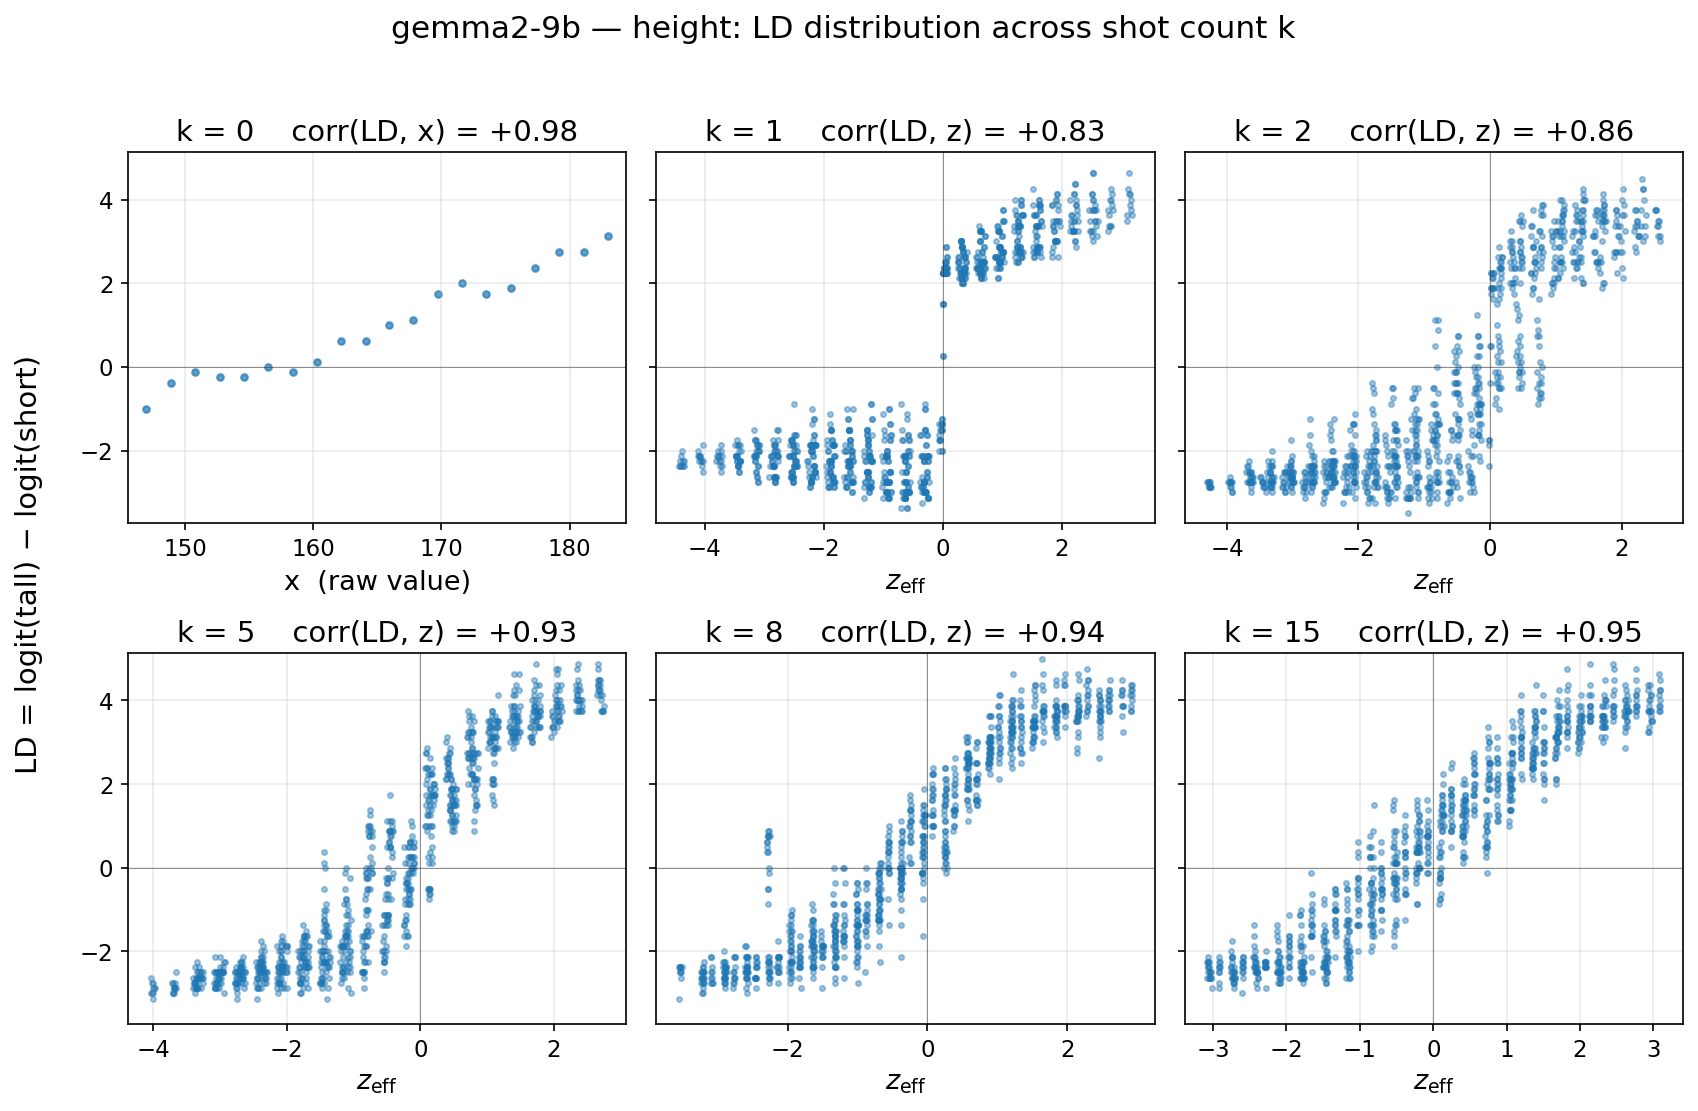
\includegraphics[width=\linewidth]{figures/p2a_ld_vs_z_height_gemma2-9b_2x3.png}
  \caption{\textbf{Logit-difference evolution with context length.}
  Without context examples, adjective judgments are driven by the raw value $x$. As context examples are added, the logit difference shifts to track relative standing, transitioning from a sharp and comparator-like step function toward a smoother and graded response.
  }
  \label{fig:kshot-ld-evolution}
\end{figure}

\Cref{fig:kshot-ld-evolution} illustrates the clear relationship between the number of context examples $k$ and how the model handles relativity. Without context examples ($k=0$), the model lacks a relative reference point and defaults to an absolute evaluation based on the raw value $x$. Providing just one example ($k=1$), however, shifts the model into a comparator-like state. The logit difference jumps sharply from $-2$ to $2$ around $z = 0$, indicating that a single comparison directly dictates the model's confidence.

As more examples are added ($k$ increases), the relationship between the logit difference and the context-normalized standing $z$ becomes smoother. For instance, at $k=15$, this relationship is nearly linear. This suggests that the model leverages the overall distribution of the provided comparison class (or performs internal comparisons across all given values) to dynamically calibrate its confidence, which is ultimately reflected in the output probabilities of the adjectives.


\begin{figure}[t]
  \centering
  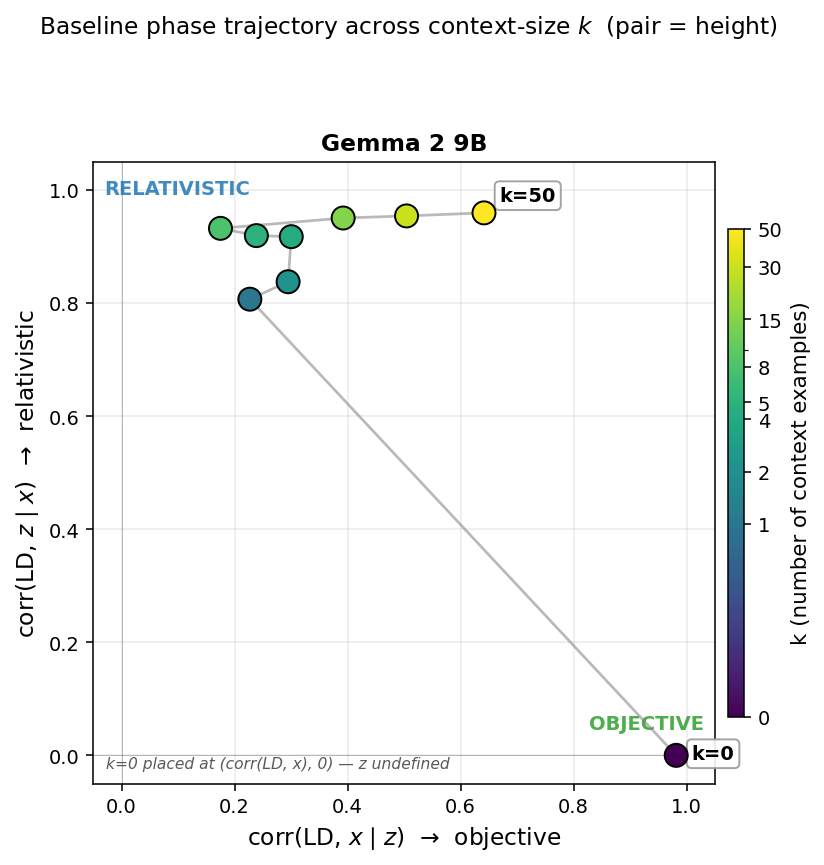
\includegraphics[width=0.9\linewidth, trim={0 0 0 80}, clip]{figures/p2d_phase_k_sweep_9b.png}
  \caption{\textbf{Relative/objective phase plane across context lengths.}
  The evolution of Gemma-2-9B model behavior as more examples are added. Providing a single context example immediately shifts the model from a highly objective state into a highly relativistic state. As more context is added, the model gradually reintegrates objective anchoring alongside its relativistic comparisons.
  % Source artifacts: internal/kshot/phase/results/p2d_l0all_per_k_gemma2-9b_height.json, p2d_partial_l0_gemma2-9b_height_k1.json, and p2e_residual_interventions_gemma2-9b_height_k15.json, replotted for paper display.
  }
  \label{fig:relative-objective-phase}
\end{figure}

In addition, since the model can rely on both the raw value $x$ and the relative standing $z$ simultaneously, we quantify the degree of objective versus relativistic behavior at each context length $k$ using partial correlations (detailed in \Cref{app:definitions}).
Specifically, \Cref{fig:relative-objective-phase} plots objective reliance measured by $\mathrm{corr}(\mathrm{LD},x\mid z)$ against relativistic reliance measured by $\mathrm{corr}(\mathrm{LD},z\mid x)$.

Without comparison context ($k=0$), variation in the adjective readout is driven primarily by the raw value $x$, though the absolute logit baseline may still reflect lexical frequency, pre-training biases, or instruction-tuning priors.
Once context is supplied ($k=1$), baseline behavior immediately shifts into the relativistic region, effectively becoming a direct comparison operation.

Surprisingly, as context length increases, the model gradually reintegrates its objective capabilities alongside the relativistic context.
This suggests that sparse numerical context typically signals a direct comparison task, whereas richer and high-context environments prompt the model to integrate the local distribution of the given values with the general distribution learned during training, allowing objective values to remain relevant.


\subsection{Sensitivity to the order of reference values}
\label{subsec:sensitivity-order}

\begin{figure}[t]
  \centering
  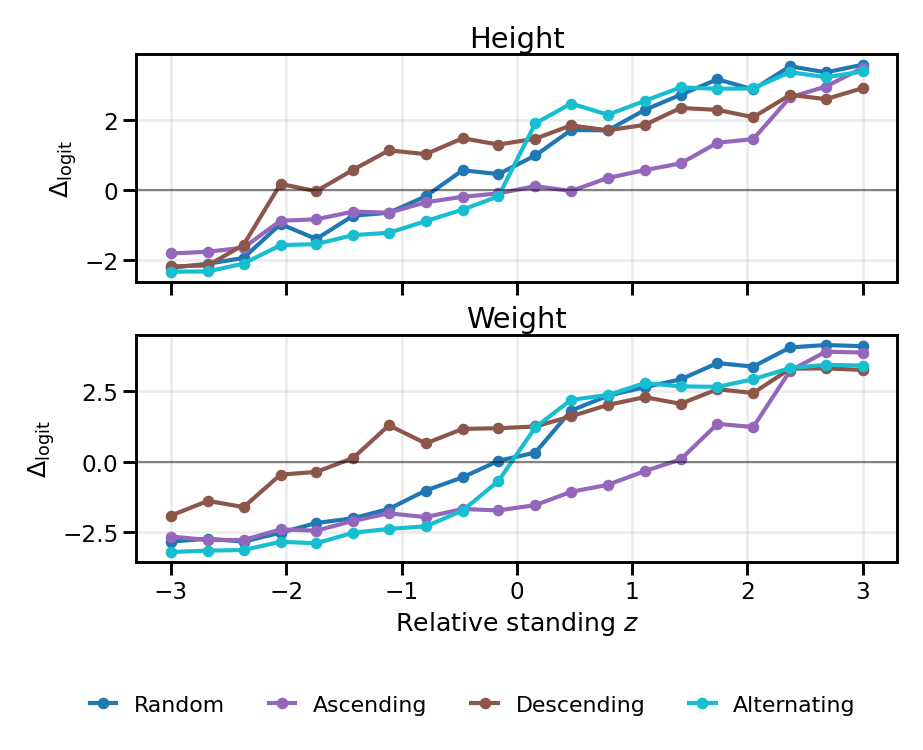
\includegraphics[width=\linewidth]{figures/fig_results_order_ld_by_z_main.png}
  \caption{\textbf{Example order modulates the relative-standing readout.}
  Logit differences plotted against $z$ under random, ascending, descending, and oscillating context orders for the height and weight concepts.
  Full eight-domain, six-order curves are shown in \Cref{fig:order-robustness-full}.
  % Source artifact: results/v14_1/order/order_rows.jsonl, replotted for paper display.
  }
  \label{fig:order-main}
\end{figure}

We next investigate whether the behavioral readout of $z$ depends on the presentation order of the context examples (e.g., random, ascending, descending, or oscillating). \Cref{fig:order-main} demonstrates that the relationship between the logit difference and $z$ is highly sensitive to this ordering.

Specifically, the model exhibits a strong recency bias, disproportionately weighting the most recently processed context values when predicting the adjective. For example, an ascending order places the highest values at the end of the context, creating a locally inflated reference class. This leads to a lower logit difference overall, as the model assigns a higher probability mass to the token ``short''.

Additionally, under an oscillating order, the logit difference exhibits a sharp jump around $z = 0$. This likely occurs because the model processes the alternating sequence as two distinct clusters, defaulting to a direct comparison between the raw value and these clusters. This mirrors the sharp, comparator-like behavior observed at $k=1$ in \Cref{fig:kshot-ld-evolution}.

Together, these findings suggest that while the model can successfully extract broad distributional statistics from the context, it heavily upweights the latest values during reasoning. This recency bias reflects human cognitive patterns, whereas one might ideally expect the model's self-attention mechanism to process context symmetrically and predict the adjective regardless of order.

\subsection{Sensitivity to the distribution of reference values}
\label{subsec:sensitivity-distribution}

\begin{figure}[t]
  \centering
  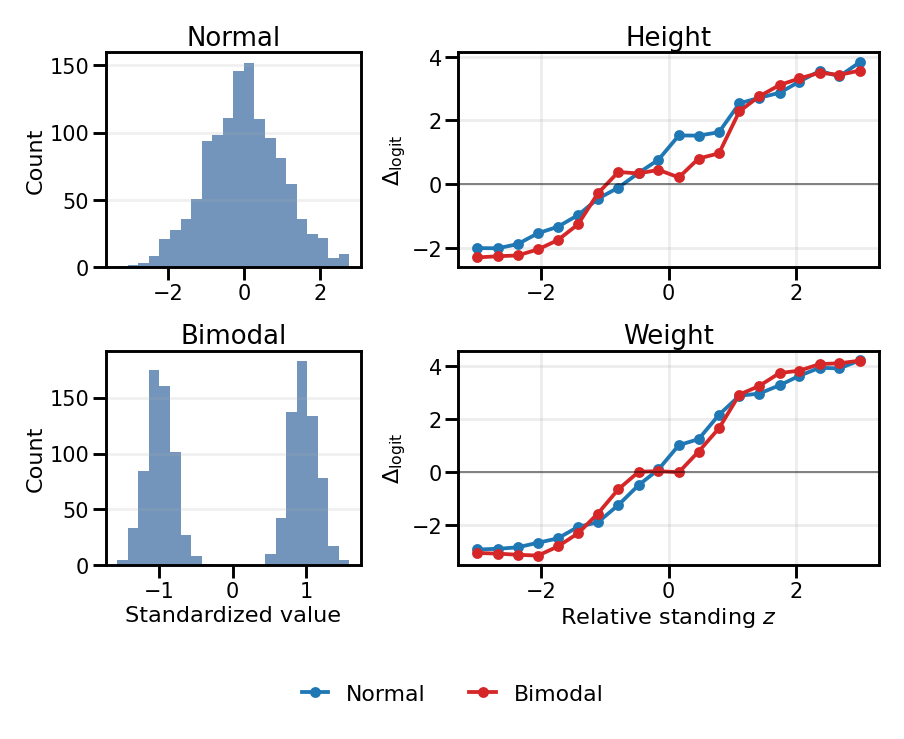
\includegraphics[width=\linewidth]{figures/fig_results_distribution_bimodal_main.png}
  \caption{\textbf{Normal and bimodal contexts yield similar relative-standing curves but distinct confidence dynamics.}
  Left: Standardized examples of context distribution shapes.
  Right: Logit difference curves against $z$ for the height and weight concepts under normal and bimodal contexts.
  % Source artifacts: results/v14/distribution/distribution_rows.jsonl and synthetic standardized shape examples, replotted for paper display.
  }
  \label{fig:distribution-shapes}
\end{figure}

Finally, we investigate how the underlying distribution of the reference values affects the relative-standing readout. \Cref{fig:distribution-shapes} compares model behavior under normal and bimodal context distributions, demonstrating that the overall trends in logit differences remain largely consistent across both shapes.

However, closer inspection reveals that bimodal distributions induce more dynamic confidence curves. Specifically, the logit difference exhibits steeper transitions around the local modes (e.g., at $z \approx -1$ and $z \approx 1$). The model outputs a lower logit difference than the normal distribution when $z$ falls just below a mode, and a higher logit difference when $z$ is just above it.

This indicates that the model evaluates the raw value relative to its closest local cluster within the context, rather than relying solely on the global mean. This behavior mirrors human cognitive patterns, where individuals naturally categorize and compare a novel observation against the most similar proximal subgroup.


\subsection{Robustness to naturalistic prompts}
\label{subsec:sensitivity-realism}

The prompts used so far present the comparison class as a terse list (``Person~1: $c_1$, \dots'').
To check that the relative-standing effect is not an artifact of this synthetic format, we re-render
each trial as naturalistic prose: the same sampled context values attached to named individuals in
full sentences (e.g.\ ``Maya is 161~cm. \dots{} Amara is 170~cm. Amara
is''), ending at the same high/low adjective cliff (\Cref{app:naturalistic-prompts} lists full example prompts). We compare two variants---a \emph{neutral}
framing that merely describes a group of people, and a \emph{primed} framing that embeds the same
values in a scenario carrying a strong absolute prior over the attribute (for height, a varsity
basketball squad).

\Cref{tab:naturalistic} reports the height pair on a dense $(x,z)$ grid, where the implicit frame
reproduces the main-text readout (corr$(\logitdiff,z)\approx0.97$; cf.\ \Cref{tab:behavioral-z-corr}).
Crucially, unlike the implicit list the naturalistic frames give no instruction to compare---the
target sentence simply states the value and stops at the adjective. Even so, the \emph{neutral}
framing stays strongly relativistic (corr$(\logitdiff,z)=0.93$), with only a modest rise in
raw-magnitude reliance (corr$(\logitdiff,x)$ from $0.13$ to $0.23$): the model uses context-relative
standing spontaneously, not because it is told to. The \emph{primed} framing, which embeds the same
values in a scenario carrying a strong absolute prior over the attribute, shifts the balance further
toward raw magnitude (corr$(\logitdiff,x)=0.45$, corr$(\logitdiff,z)=0.84$), though relative standing
still dominates. The model thus integrates in-context standing with world knowledge: realistic
phrasing alone does not weaken the relativistic computation, but a framing that makes absolute scale
salient shifts the objective/relativistic balance, echoing the reintegration of objective anchoring
observed at high context length (\Cref{fig:relative-objective-phase}).

\begin{table}[t]
  \centering
  \footnotesize
  \setlength{\tabcolsep}{4pt}
  \caption{\textbf{Relative-standing dominance survives naturalistic prompts (height).}
  Correlations of the mean logit difference with the context-normalized standing $z$ and the raw
  value $x$ on a dense $(x,z)$ grid. Naturalistic-neutral prose stays strongly $z$-dominant even
  without a comparison cue; a framing that invokes a strong absolute prior (a basketball squad)
  shifts weight toward $x$.}
  \label{tab:naturalistic}
  \begin{tabular}{lrr}
    \toprule
    Prompt frame & corr$(\logitdiff,z)$ & corr$(\logitdiff,x)$ \\
    \midrule
    Implicit list (main text) & \textbf{0.966} & 0.130 \\
    Naturalistic, neutral     & \textbf{0.926} & 0.233 \\
    Naturalistic, primed      & \textbf{0.844} & 0.450 \\
    \bottomrule
  \end{tabular}
\end{table}



\section{Mechanistic Results}
\label{sec:mechanistic-results}
We now investigate how the internal representations of LLMs encode the raw numerical value ($x$) and the context-normalized standing ($z$).

\subsection{Relative standing is linearly encoded}
\label{subsec:layer-evolution}

\begin{figure}[t]
  \centering
  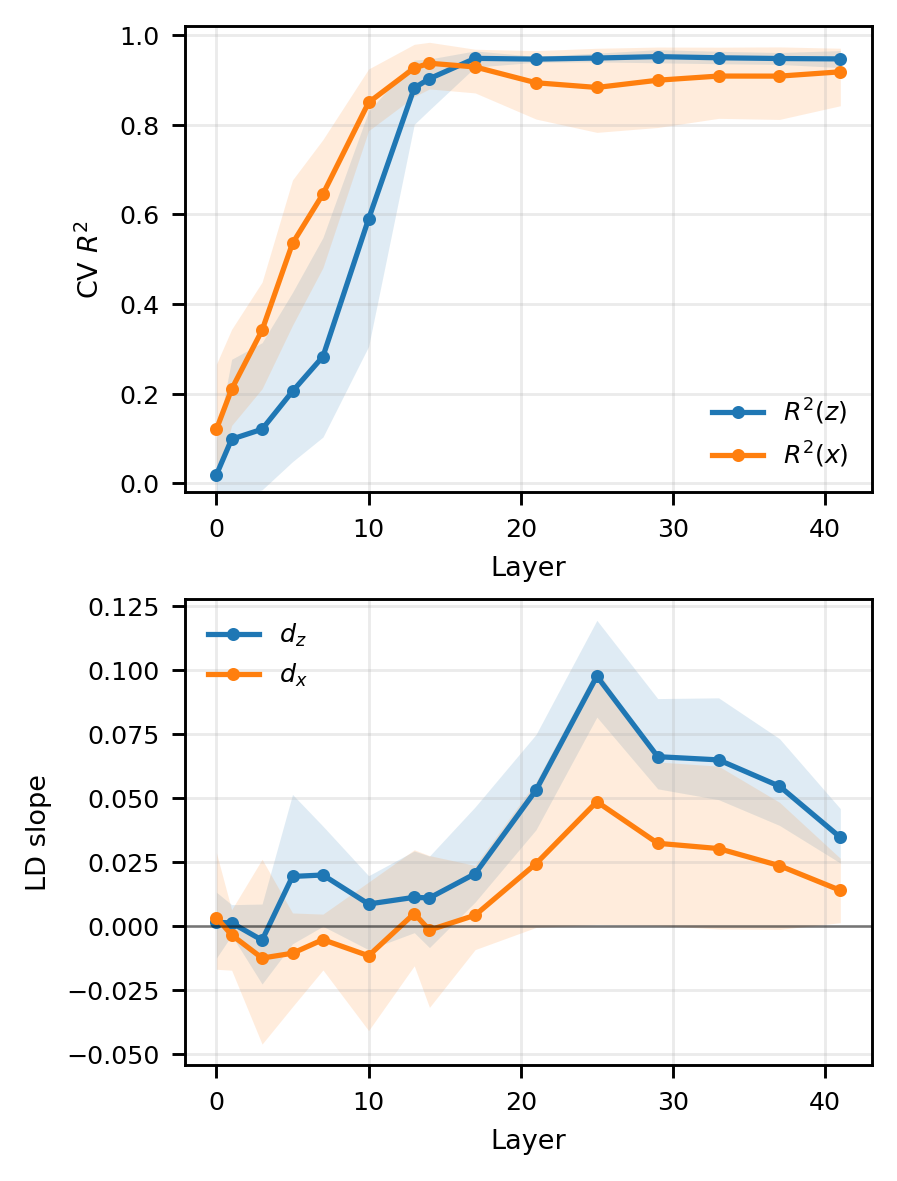
\includegraphics[width=\linewidth]{figures/fig_results_layer_z_x_encode_use_clean.png}
  \caption{\textbf{Both $z$ and $x$ are linearly encoded, but direct steering on $z$ at middle layers is the most effective.}
  In Gemma-2-9B, cross-validated linear probes decode both the relative standing $z$ and raw magnitude $x$ across layers (top).
  Direct steering has a substantially larger late-layer effect along \primalz{} than along \primalx{} (bottom).
  % Source artifact: results/v14_1/fig5/fig5_layer_x_z_metrics.json, replotted for paper display.
  }
  \label{fig:layer-encode-use}
\end{figure}

For each adjective pair and layer $L$, we fit ridge linear probes from residual-stream activations to the target variables $x$ and $z$.
The reported cross-validated $R^2$ uses five shuffled folds: each probe is trained on four folds, evaluated on the held-out prompts, and scored from the aggregate out-of-fold predictions.
The top plot in \Cref{fig:layer-encode-use} illustrates that both the raw value $x$ and the relative standing $z$ are linearly decodable from the model's representations.
Notably, $x$ is more strongly represented in the earlier layers, whereas $z$ becomes highly decodable in the later layers.
This suggests a sequential processing dynamic: the model initially processes the raw value $x$, and subsequently computes the relative standing $z$ once contextual information has been integrated.

The bottom plot demonstrates that steering the residual stream along mean difference direction \primalz{} shifts the adjective logit difference. The effect size of this intervention, measured by the steering slope, tends to be large precisely when the linear decodability (measured by $R^2$) is high. Specifically, steering along \primalz{} achieves its maximum impact when applied around layer 25.

Although intervening on the raw value direction \primalx{} also influences the output, modifying the relative standing directly is substantially more effective. Because successful linear probing only indicates decodability rather than definitive proof of a causal feature, this steering result is crucial; it provides causal evidence that the model actively relies on the \primalz{} direction to formulate its adjective predictions.



\subsection{A Shared $z$ Direction Across Concepts}
\label{subsec:shared-direction}
\begin{figure}[t]
  \centering
  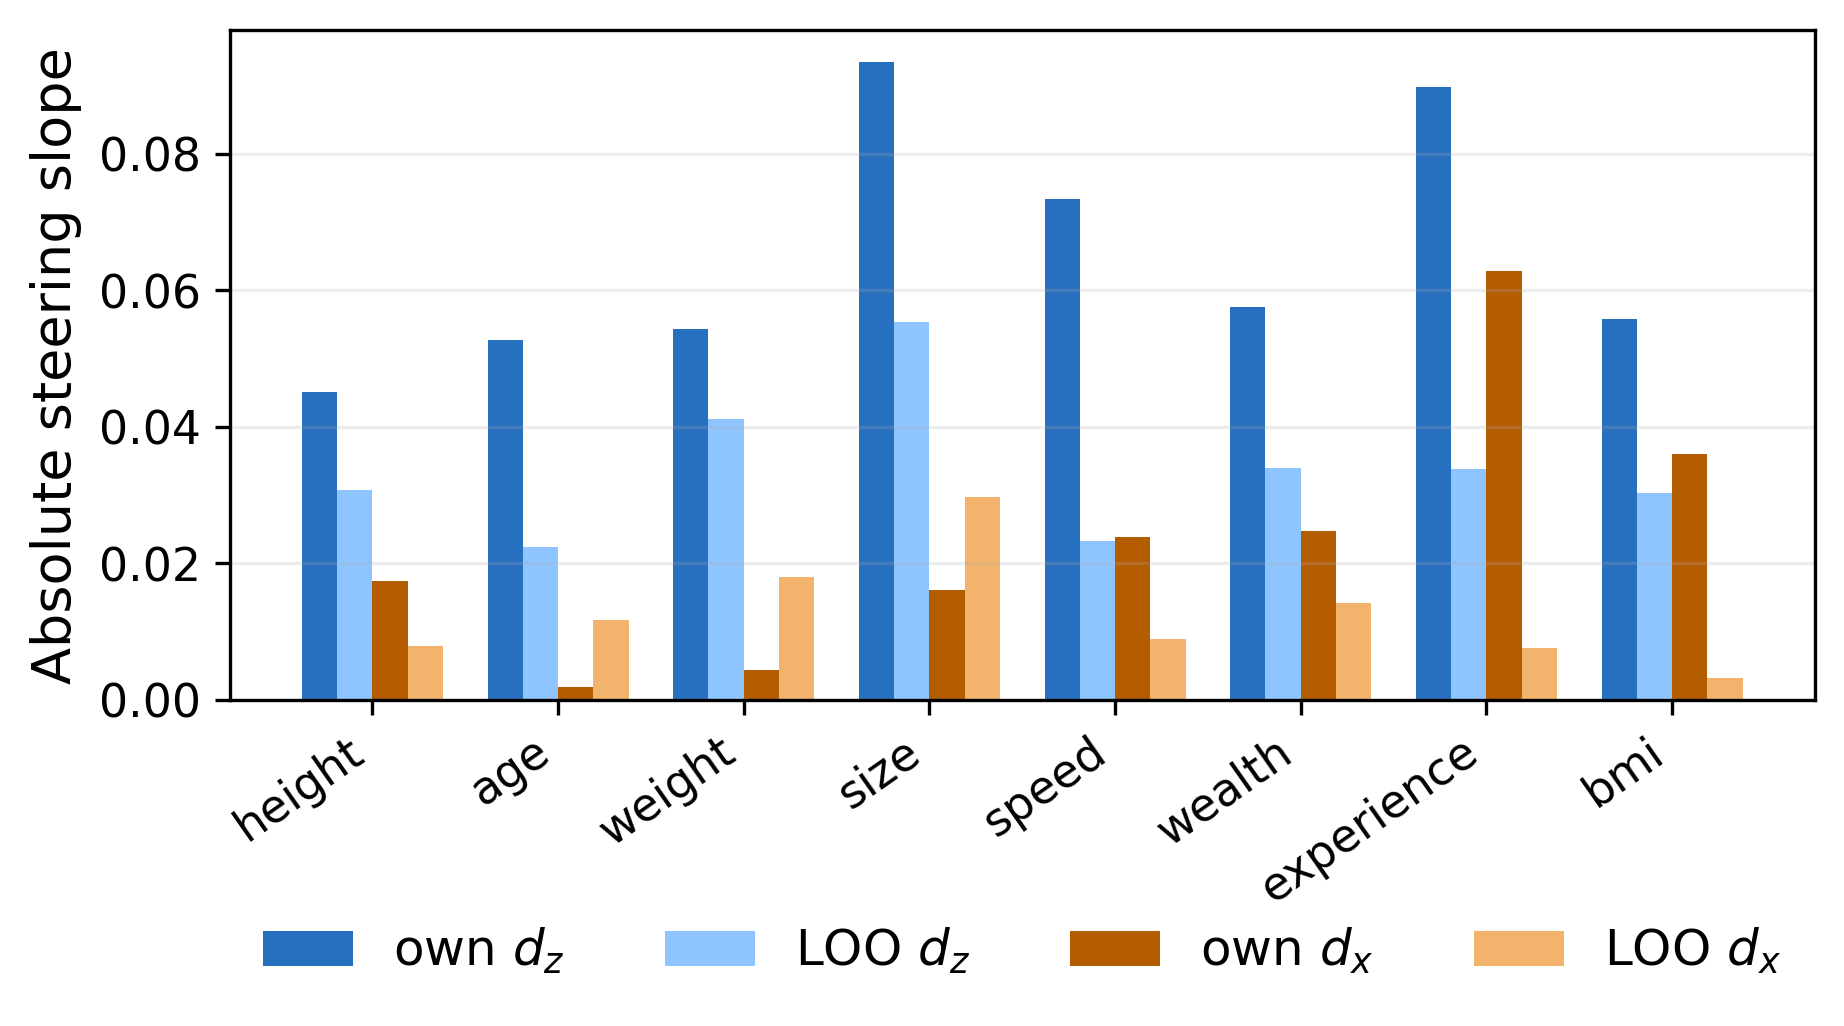
\includegraphics[width=\linewidth]{figures/fig_results_shared_direction_own_loo_abs_slopes_z_vs_x.png}
  \caption{\textbf{Leave-one-out shared directions preserve much of \primalz{}
  steering.}
  For Gemma-2-9B at layer 33, bars show absolute steering slopes for each
  concept's own direction and for a leave-one-out (LOO) shared direction built
  from the other seven concepts.
  LOO \primalz{} retains a substantial fraction of own-\primalz{} steering,
  whereas raw-\primalx{} effects are generally weaker and less consistently
  shared. % Source artifact: results/v15/shared_direction_loo_z_vs_x.json, replotted
  % for paper display.
  }
  \label{fig:shared-direction-steering}
\end{figure}

We next ask whether each adjective pair has its own individual direction, or whether a shared $z$-like relativity component transfers across concepts.

For each adjective pair, we compute a \primalz{} direction as the difference between mean residual-stream activations for high-$z$ and low-$z$ prompts.
We form a leave-one-out shared direction for each held-out target by sign-aligning and averaging the other seven \primalz{} directions, and apply the same construction to raw-value directions \primalx{}.
\Cref{fig:shared-direction-steering} shows that the shared \primalz{} directions recover a substantial fraction of own-concept steering, suggesting that relative standing is partly represented in a common residual-stream direction rather than only in concept-specific axes.
The raw-\primalx{} comparison is weaker and less systematic: some domains show nonzero magnitude directions, but these directions do not provide the same consistent shared steering signal.
\Cref{fig:z-vs-x-transfer} provides the complementary full cross-pair transfer matrix. We see that transferability is substantially stronger for \primalz{} than for raw-$x$ directions.


\subsection{Manifold Steering Preserves Objectivity} 
Research has demonstrated that better intervention results can be achieved by steering along higher-dimensional latent structure rather than a single linear direction~\citep{sarfati2026beliefs}. We apply manifold steering in our setting by estimating a discrete vector field over $(x,z)$ from mean residual activations, then iteratively transporting activations toward neutral relativity ($z\approx0$) within each fixed-$x$ slice. A full algorithm is found in \cref{alg:manifold-arclength}.

\begin{figure}[t]
  \centering
  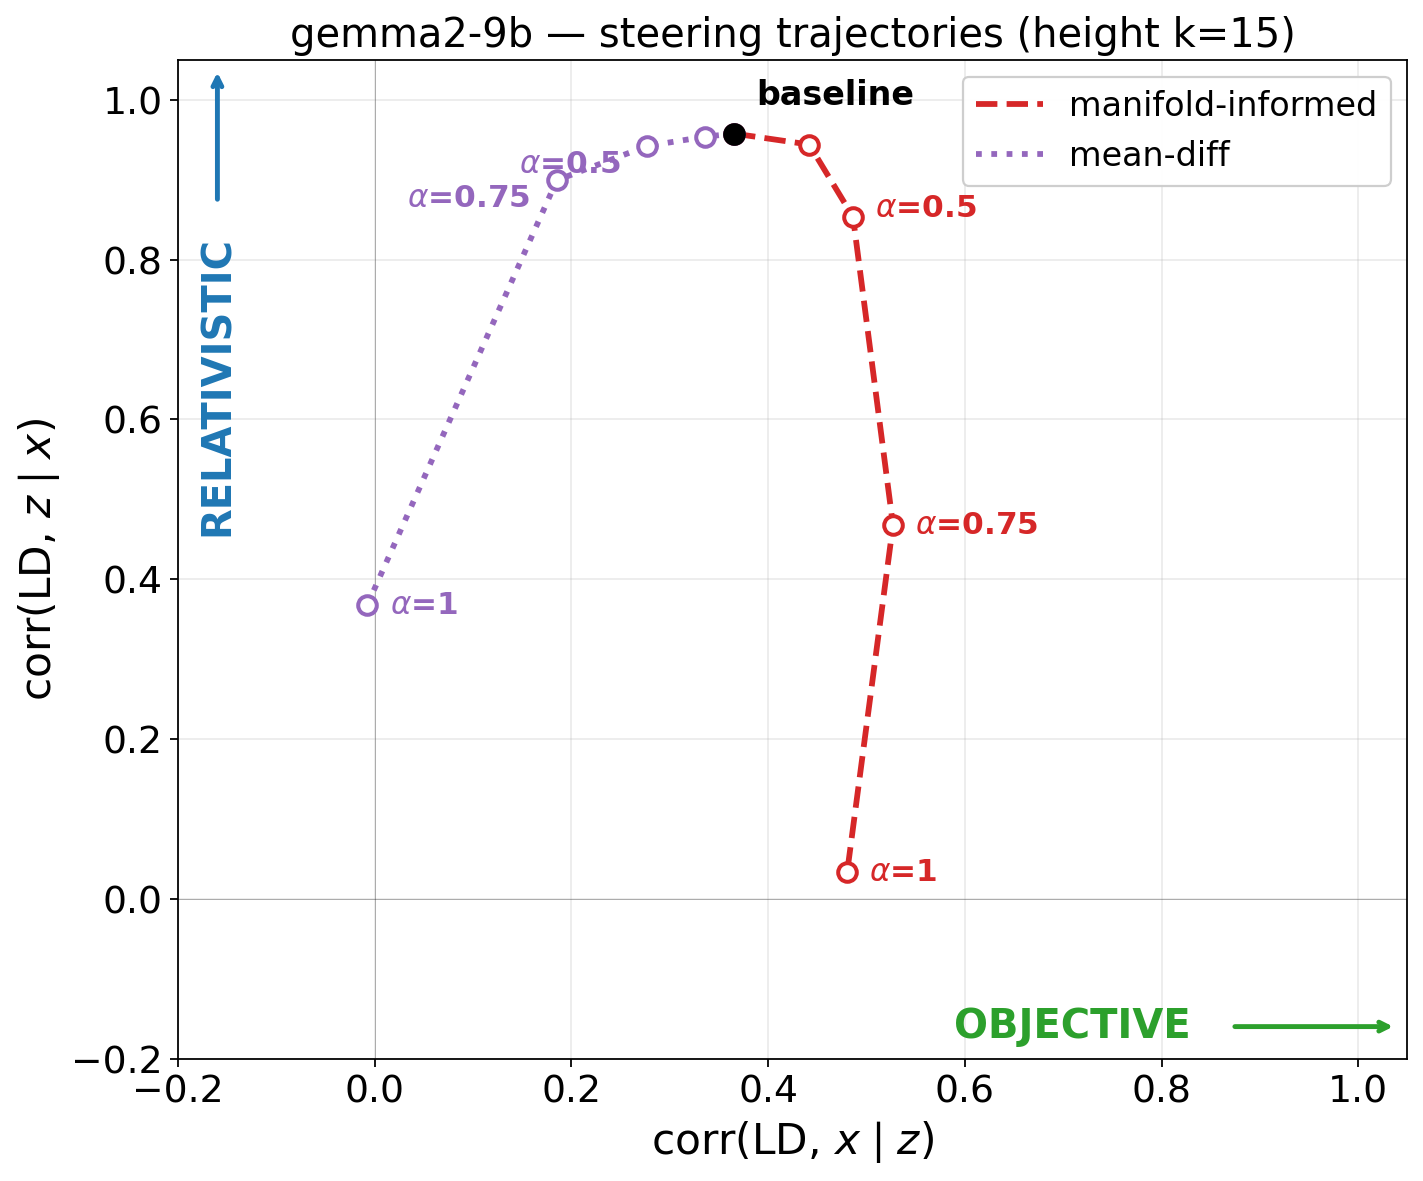
\includegraphics[width=\linewidth]{figures/p2v_steering_with_arclength_gemma2-9b_height.png}
  \caption{\textbf{Manifold informed and mean diff steering trace different routes out of the relativistic region on Gemma-2-9B.}
  % Source artifact: relativity_ablation/figures/p2v_phase_trajectory_partial_gemma2-2b.png.
  Steering conducted at L33. We see manifold based steering much better at isolating the relativistic direction.
  }
  \label{fig:circuit-phase-trajectory}
\end{figure}

Results from this steering method compared to mean diff $d_z$ steering are displayed in \cref{fig:circuit-phase-trajectory} for height, with k=15 shot context. Manifold-informed steering indeed is much stronger at univariately ablating relativistic behavior while preserving objective capabilities of the model, which the $d_z$ steering destroys. 


\paragraph{Steering Conclusions}
Steering interventions show that the concept of $z$ and thus relativity is linearly decodable and furthermore partially transfers across gradable adjectives. However, a linear decomposition of the relativity feature as is done in $d_z$ confounds the features of relativity and objectivity, destroying both. Manifold-based steering is able to solve this, effectively isolating the relativity feature through steering $(x,z)$ pairs towards $(x,0)$. 

\subsection{Attention Based Interventions Transfer}
\label{subsec:attention}

Alongside conventional intervention methods such as mean-diff and manifold steering, we also demonstrate causality in attention-based interventions in Gemma-2-9B. We experiment with choosing heads based on direct-logit-attribution (DLA) \citep{elhage2021transformer} scoring as well as cosine-similarity scoring to relativity as a direction expressed in $d_{z,L}$ space. In particular, ablating a small number of heads (e.g. 5 out of a total 672) can strongly reduce the relativity readout to logits while achieving minimal KL divergence on normal natural language prompts and other linearly based features. The same heads transfer across multiple tested gradable adjective concepts.

Appendix~\ref{app:attention-details} details the ranking definitions, while \Cref{fig:intervention-modes,fig:ranking-comparison} show their performance. For the purposes of this paper, ``ablation'' refers to heads chosen via DLA whose $\mathrm{softmax}(QK^T/\sqrt{d}) V$ vectors are resampled from other prompts of different $(x,z)$ before being concatenated and multiplied by $W_O$.

\cref{fig:circuit-trio} shows the cumulative effects of Greedy top-$N$ head resampling ablation under DLA ranking, driving $corr(\mathrm{LD}, z)$ from $+0.93$ through zero to $-0.12$ by $N{=}10$ on Gemma-2-9B (height, $k{=}15$). We also display on the right axis the cosine alignment of the $\Delta h_L$ after a head is ablated to $d_{z,L}$, providing a clear intuition as to what the ablation is doing. In these specific heads, resampling their attention calculations is very similar to steering them towards the opposite end of their relativity internal representation, providing causal evidence that these heads are responsible in part for the mid layer relativity computation we observed earlier. 

\begin{figure}[!tbp]
  \centering
  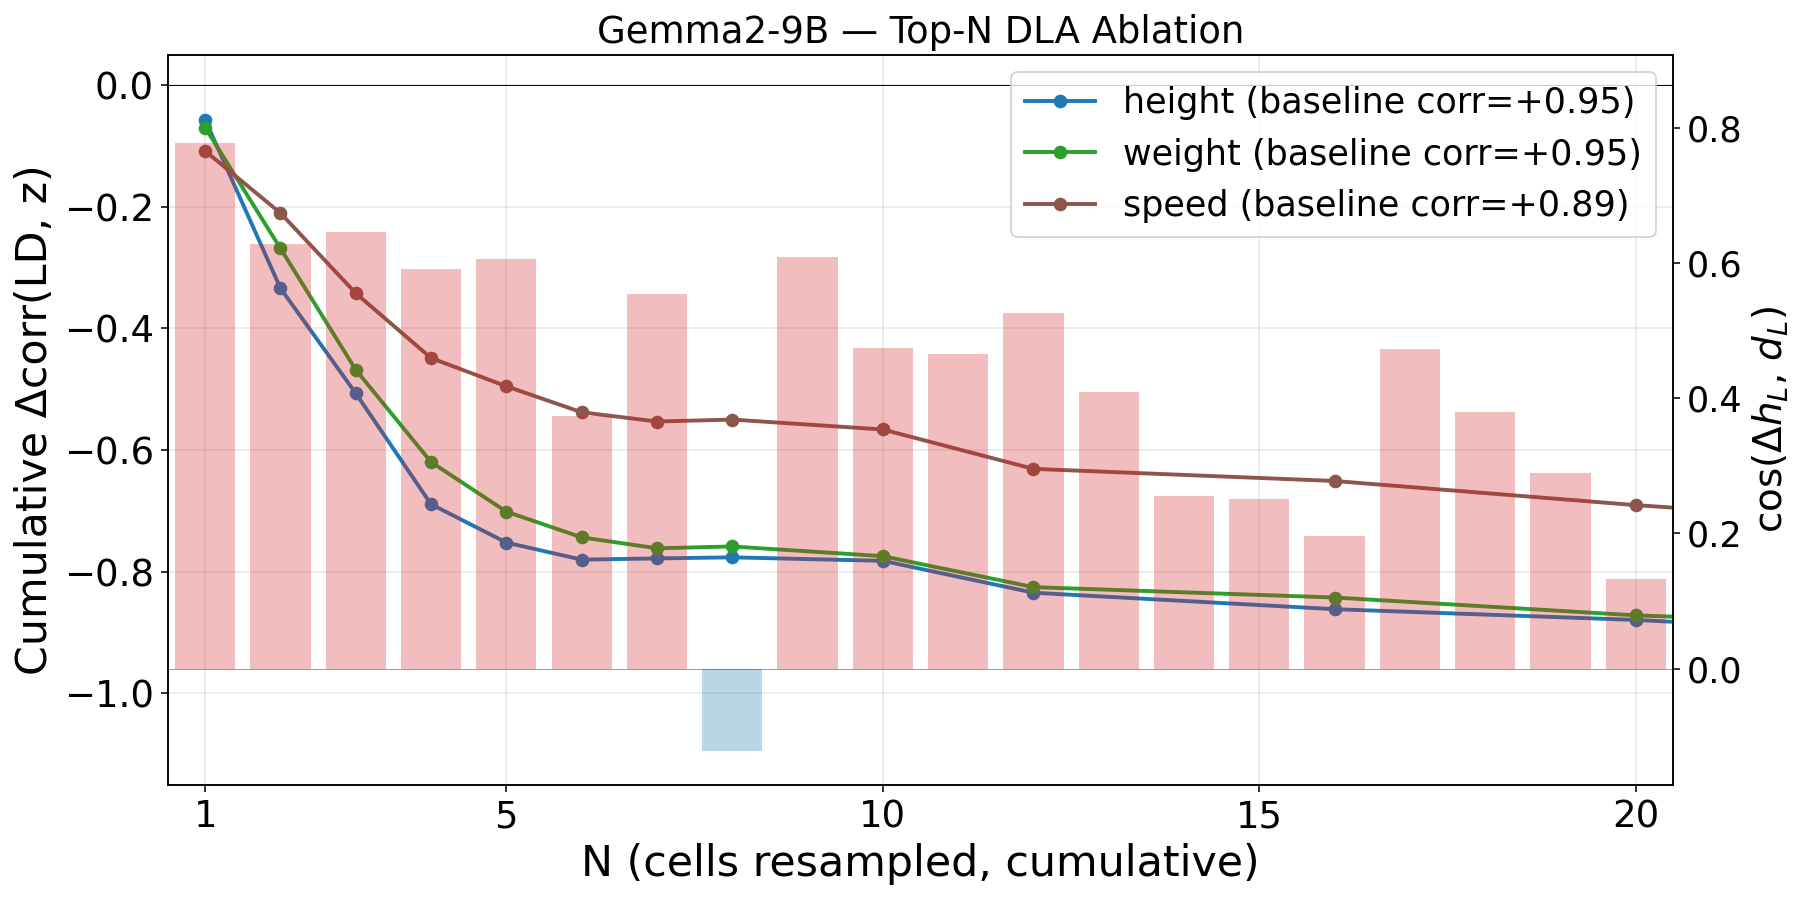
\includegraphics[width=\linewidth,trim=0 0 0 0,clip]{figures/p2u_n_sweep_xfeat_gemma2-9b_dcorr.png}
  \caption{\textbf{DLA-ranked greedy ablation drives the model's relativity alignment to zero on Gemma-2-9B.}
  Left axis: Cumulative $\Delta corr(\mathrm{LD},z)$ over top-$N$ greedy resampling under DLA ranking using only HEIGHT prompts.
  Right axis: Cosine similarity of the hidden layer activation differences under ablation to the relativity vector $d_z$ for newly added cells.
  Height derived DLA heads generalize to other relativity concepts, with a near perfect transfer to weight and a partial transfer to speed.
  % Source artifact: relativity_ablation/figures/p2u_n_sweep_xfeat_gemma2-2b-it.png.
  }
  \label{fig:circuit-trio}
\end{figure}

Further supporting this claim is the fact that these heads generalize remarkably well across different adjective pairs, also shown in \cref{fig:circuit-trio}. The joint resample of L23H14, L26H4 and L31H3 (Top 3 heads under height) drops $r(\mathrm{LD}, z)$ by $0.51$ on height, $0.47$ on weight, and $0.34$ on speed --- $39$--$53\%$ of the baseline correlation in each case --- indicating that the circuit is relativity-general rather than tied to any one surface adjective, and like steering also partially transfers. Applying DLA natively to speed and weight produces a very similar head ranking, as shown in \cref{fig:fingerprint}.

This transfer also scales across different k-shot prompting, as shown in \Cref{fig:xk-corr-grid-9b-height,fig:xk-deltar-overlay-9b-height}, which replicates the height attention ablation to k=1 and k=5. The objective and relativistic plane figures also provide another mechanistic lens as to how similar the attention based ablations are to $d_z$ steering.

The trio is also robust to the prompt format itself. Re-running the resample ablation on the naturalistic, prose-framed prompts of \Cref{subsec:sensitivity-realism}---named individuals with no explicit instruction to compare---still collapses the readout, dropping $\mathrm{corr}(\mathrm{LD},z)$ from $0.74$ to $0.36$ on height ($\Delta r = -0.38$), paralleling the $-0.52$ drop the same trio produces on implicit-list prompts over this grid. The circuit mediating the relativistic computation is therefore not an artifact of the synthetic list format.

\begin{figure}[!tbp]
  \centering
  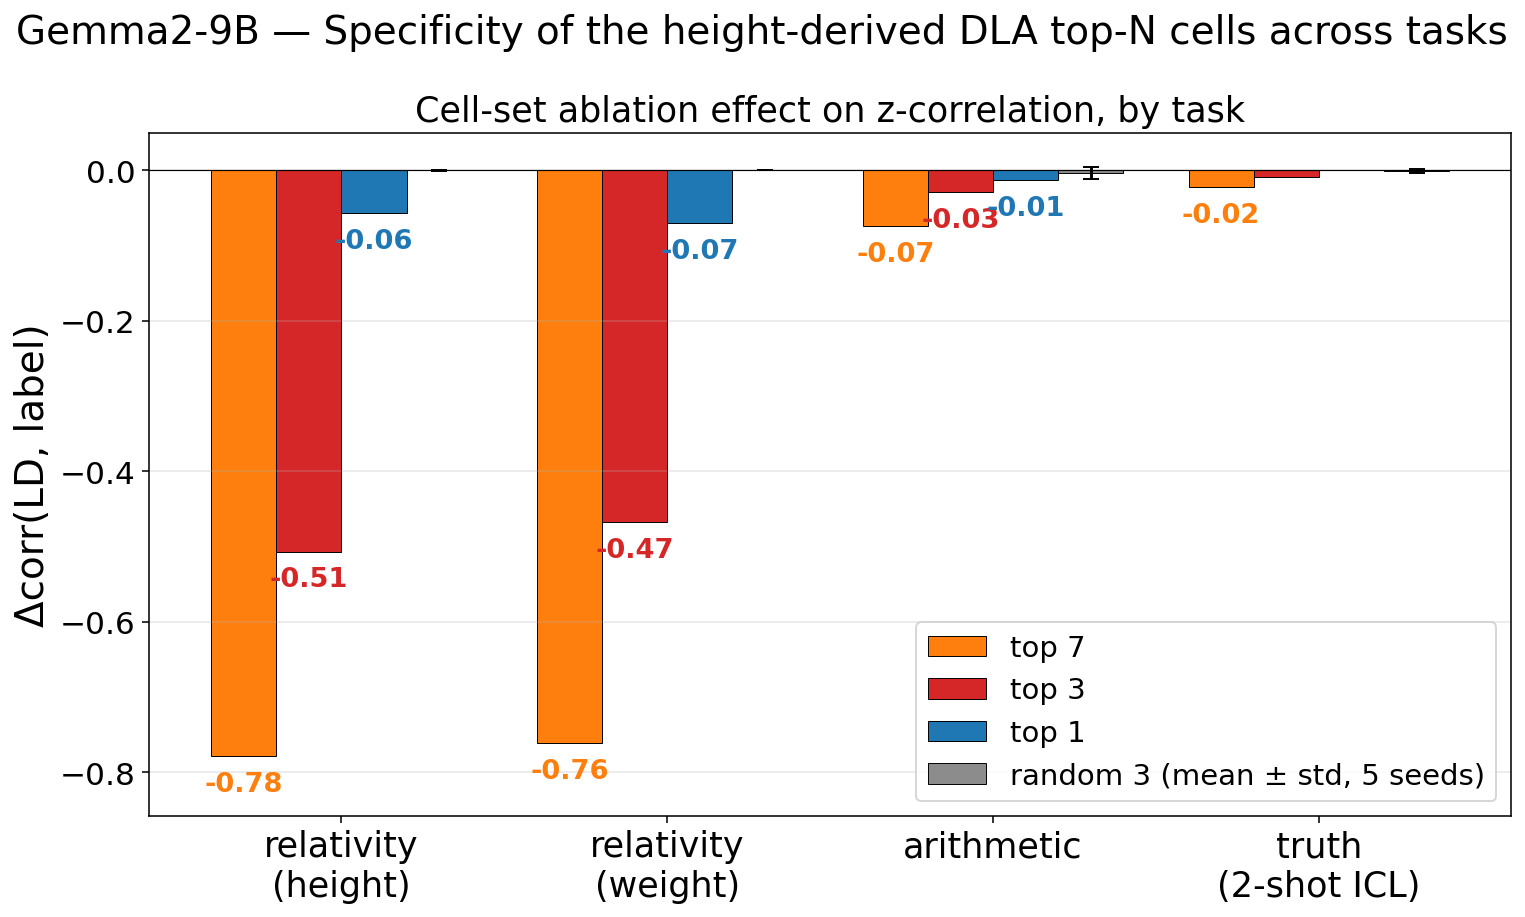
\includegraphics[width=\linewidth,trim=0 0 0 0,clip]{figures/p2u_specificity_summary_gemma2-9b_dr.png}
  \caption{\textbf{Specificity of height derived heads}
  We see that heads produced by DLA ranking on height are remarkable at ablating away the correlation between LD of adjectives and their Z score. For arithmetic and truth, correlation was measured between the LD of "True" and "False" against the true label. This calculation was largely unaffected by the ablations on height derived heads. Baseline correlations for all tasks are $> 0.95$. Heads were resampled based on their own task prompt sets. 
  % Source artifact: relativity_ablation/figures/p2u_n_sweep_xfeat_gemma2-2b-it.png.
  }
  \label{fig:circuit-spec}
\end{figure}

To test whether the trio simply damages general competence, we ran the same intervention on arithmetic comparison ("Is X $>$ Y"), factual truth ("Paris is the capital city of France") \citep{marks2023geometry}, and raw natural-language imperatives. In each case, we again resample the attention head outputs from each prompt set to corrupt the residual stream at these heads. Results are shown in \cref{fig:circuit-spec}. Specificity is sharp: trio $\Delta corr$ is $-0.03$ on arithmetic and $-0.01$ on truth, and raw-text KL is indistinguishable from random three-head ablation ($0.009$ vs.\ $0.008 \pm 0.004$ nats); the relativity/neutral KL ratio is $17\times$ at $N{=}3$. KL curves of relativity features against natural language are shown in \cref{fig:kl}.

\paragraph{Attention Conclusions}
Our attention based ablations demonstrate evidence that certain heads are heavily relied upon for the computation of relativity in Gemma-2-9B. Generally, residual information about relativity is dispersed very broadly throughout the layers and heads of the transformer, such that under random corruption of heads the relative readout of an $(x,z)$ pair is able to be preserved and recovered. However, a joint corruption of a few heads chosen by DLA is able to produce an unrecoverable effect on relativity calculations that is very similar to mean diff steering, destroying the partial correlation between $LD$ and $z$ given $x$. This same circuitry appears to generalize well to other relativistic concepts, but not to other linear features and natural language, showing a degree of specialization. This evidence suggests that in Gemma-2-9B, certain heads are causally significant for encoding something akin to the relative standing of $z$.


\subsection{Generalization Across Model Scale}

The main behavioral decomposition into $z$-score relativity and dense-grid behavior was replicated across several small model families, including OLMo 2 7B, Pythia 2.8B, Llama 3.2 3B, Qwen 2.5 3B, and Qwen 3 14B; appendix cross-model summaries are shown in \Cref{fig:xmodel-geometry,fig:xmodel-interventions}.

The broader generalization question to larger models with more parameters remains largely open. The largest model we tested was 14B parameters.


\section{Discussion and Related Work}
\label{sec:discussion-related-work}
\label{sec:related-work}


% We show that in-context scalar judgments on relative gradable adjectives are better described by a context-normalized variable than by raw magnitude alone.
% Behaviorally, the dense grid and robustness controls show $z$-dominant behavior across ordinary, reordered, non-Gaussian.
% Internally, PCA shows activation geometry, steering shows causal use, and attention interventions identify a small set of heads that can strongly reduce the relativity readout.

% The shot-sweep phase result adds a behavioral refinement: with no comparison examples, the model behaves more like an objective magnitude reader, but even one context example moves it toward a relative judgment regime.
% This suggests that the model is not merely retrieving a fixed pretrained prior, but is dynamically changing the internal computations as the prompt supplies more examples.

% Intervention results strengthen this view. \primalz{} steering and dual steering shift adjective decisions along the relative axis.
% Cross-concept transfers are stronger for \primalz{} than raw-$x$ directions, and lexical decomposition shows that the lexical residuals preserve more off-diagonal transfers than pure adjective-specific lexical projections.
% 

% Taken together, these results suggest that comparison examples induce a $z$-like representation that is visible in outputs, residual-stream geometry, steering effects, and attention interventions.
% Relativity is therefore internally represented and causally relevant, but it is not implemented by a single one-dimensional vector: lexical structure, shared residual directions, and attention-mediated routing all contribute to the mechanism.

\subsection{Gradable Adjectives and Pragmatic Thresholds}
\label{subsec:related-gradability}

Before modern LLMs, a general pragmatic understanding of relative gradable adjectives in natural language was studied. \citet{lassiter2017adjectival} provide a Bayesian framework for interpreting this class of adjectives. Recent LLM work and the discovery of in-context learning further test the inferential capabilities of Bayesian pragmatic models \citep{lipkin2023pragmatic}. Our work, built on these foundations, extensively focuses on interpreting how the comparisons and relativity are geometrically represented in the model's internal representations.

\subsection{Numerical Representations and In-Context Statistics}
\label{subsec:related-numbers}

Prior work has shown that language models can encode numerical magnitude \citep{zhu2024value}. This literature mainly targets raw magnitude: whether the model can represent that one number is larger than the other. Our setting extends this concept but moves to a richer setting, whether a target value is high or low relative to the distribution implied by the prompt, and whether language models are able to encode this relativity internally.

This also connects to work explaining in-context learning phenomena as statistical inference, where language models infer the task-relevant structure from examples in the prompt \citep{xie2022implicitbayesian,he2025linearregression}. Our setting differs in one important way, as the examples are sampled scalar values drawn from a parameterized population distribution, rather than explicitly instructing the model to compare examples.

\subsection{Linear Representations, Steering, and Manifold Geometry}
\label{subsec:related-mi}

Linear representations of natural-language concepts are a common starting point for mechanistic interpretability \citep{park2024linear,park2025categorical}; linear methods such as probing and steering are often used to connect the geometry of the linear representation to the behavior of the model.
However, more recent work shows that not all features are well described by a one-dimensional linear direction; certain features appear to require richer geometry such as cyclical, hierarchical, and low-dimensional manifold structure \citep{engels2024notlinear,modellerubin2025manifolds,sarfati2026beliefs,gurnee2026manifold}.

Our use of \primalz{} sits between these views. Concepts such as \emph{tall} vs \emph{short} could be interpreted as counterfactual or binary which is best represented linearly, whereas other interpretations might suggest it is based on a probability distribution which is represented in nonlinear manifolds \citep{sarfati2026beliefs, park2026softmaxgeometry}. Therefore, while testing linear decodability and steerability and the downstream causal effects of $z$, we also deploy methods such as manifold steering to test whether nonlinear geometry matters, without reducing the mechanism into a single ``the model has a vector'' claim.

\subsection{Limitations and Future Work}

Several limitations remain. First, the main methodology in constructing the behavioral readout is a high-minus-low logit difference over hand-chosen adjective tokens.
More robust settings would include a broader set of synonym/antonym families and a deeper analysis of top-logit behavioral changes.
Secondly, the chosen domains are mostly drawn from human-interpretable quantities such as weight, height, and size.


The attention intervention experiment is not yet a complete circuit-level explanation.
While it identifies important heads with causal evidence through greedy ablation, it does not decompose the full algorithm by which the model estimates the comparison statistic from context.
In particular, we do not yet know how or whether the model explicitly represents $\mu$ and $\sigma$, processes the normalized statistic to downstream layers, or approximates the same behavior through a more distributed comparison process.
Future work should test broader lexical readouts, semantically distant scalar domains, and circuit-level decompositions of how comparison statistics are formed and routed.


\section*{Impact Statement}

This paper aims to advance mechanistic understanding of how large language models use context when making scalar judgments.
It studies synthetic prompt tasks and does not introduce a deployed model, personal dataset, or decision procedure.
The main potential benefit is methodological: the experiments provide a controlled way to distinguish raw numerical magnitude, context-normalized standing, linear decodability, causal steering, and attention-based intervention effects, which may help future interpretability work in similar settings.

The topic has potential relevance to AI safety and fairness, as many real applications involve context-sensitive scalar comparisons.
Mis-specified comparison classes could produce misleading or unfair judgments, especially in high-stakes domains. 
Our results should therefore not be read as evidence that current models make reliable or fair context-sensitive decisions in deployment. 
Any such use would require domain-specific validation, careful choice of reference classes, and safeguards against harmful comparisons.

\bibliography{references}
\bibliographystyle{icml2026}

\appendix
\crefalias{section}{appendix}
\onecolumn

\section{More Definitions and Metrics}
\label{app:definitions}
\paragraph{Squared-correlation $R^2$.}
Unless explicitly marked as a cross-validated probe score, reported $R^2$ values are squared correlations:
\[
R^2(a,b)=\mathrm{corr}(a,b)^2.
\]

\paragraph{Partial correlation.}\label{app:partial-corr}
For scalar variables $a,b,c$, the (Pearson) partial correlation is defined as
\[
\mathrm{corr}(a,b \mid c)
=
\frac{
\mathrm{corr}(a,b) - \mathrm{corr}(a,c)\,\mathrm{corr}(b,c)
}{
\sqrt{(1-\mathrm{corr}(a,c)^2)(1-\mathrm{corr}(b,c)^2)}
}.
\]
Equivalently, it can be computed by removing the linear component of each variable along $c$, i.e.
\[
a^\perp = a - \hat a(c), \quad b^\perp = b - \hat b(c),
\]
where $\hat a(c)$ and $\hat b(c)$ are least-squares projections onto $c$, and then computing
\[
\mathrm{corr}(a,b \mid c) = \mathrm{corr}(a^\perp, b^\perp).
\]
Intuitively, this measures the correlation between $a$ and $b$ after projecting out their shared linear component along $c$.

% \paragraph{PCA $R^2$.}
% PCA is fit to activation vectors $h_i\in\mathbb{R}^d$.
% For a principal direction $v_{\mathrm{PC1}}$, each example receives a scalar score
% \[
% s_i=(h_i-\bar h)\cdot v_{\mathrm{PC1}}.
% \]
% Then $R^2(\mathrm{PC1},z)=\mathrm{corr}(s,z)^2$.
% This is not PCA explained variance; it asks whether position along a PC orders examples by $z$.




% \section{Lexical Decomposition}
% \label{app:lexical-decomposition}

% For each pair, lexical directions are built from token-position captures such as adjective-token states, adjective-in-sentence states, sentence-final states, synonym-token contrasts, and domain-token contrasts.
% Token-position captures use tokenizer offsets to average hidden states over the tokens overlapping the relevant word or phrase.
% These directions form an orthonormal lexical basis:
% \[
% Q_L=\operatorname{orth}([d_1,\dots,d_k]).
% \]
% Normalize the context direction:
% \[
% p_z=\operatorname{unit}(\primalz).
% \]
% Project into the lexical subspace and take the residual:
% \[
% p_{z,\mathrm{lex}}=Q_LQ_L^\top p_z,\qquad
% p_{z,\mathrm{resid}}=p_z-p_{z,\mathrm{lex}}.
% \]
% By construction, $p_{z,\mathrm{lex}}^\top p_{z,\mathrm{resid}}\approx 0$.
% The lexical energy fraction is $\|p_{z,\mathrm{lex}}\|^2$ because $p_z$ is unit norm.

% Steering uses normalized versions of the projection and residual.
% Therefore a small lexical projection can steer more strongly than full \primalz{} if it points in a high-gain output-facing direction.
% In the current 9B layer-33 follow-up, full \primalz{} has diagonal/off-diagonal means $+0.067/+0.026$, lexical projection has $+0.087/+0.011$, lexical residual has $+0.044/+0.024$, and a random null is approximately zero.
% This supports a mixed mechanism: the residual carries broad cross-domain transfer, but target lexical-subspace leakage prevents a clean non-lexical claim.


\section{Naturalistic prompt examples}
\label{app:naturalistic-prompts}

The robustness check in \Cref{subsec:sensitivity-realism} re-renders each trial as naturalistic
prose, holding the sampled context values, the implied $(\mu,\sigma)$, and the high/low adjective
cliff fixed; only the surface framing changes. Representative prompts follow for the height pair at
$k=6$ context examples (implicit list, neutral naturalistic, and primed naturalistic), plus a primed
income example. In every case the target value---and hence $z$---is identical across frames.

\paragraph{Height, implicit list (main text).}
{\small\begin{verbatim}
Person 1: 157 cm
Person 2: 165 cm
Person 3: 158 cm
Person 4: 157 cm
Person 5: 151 cm
Person 6: 158 cm
Person 7: 170 cm. This person is
\end{verbatim}}

\paragraph{Height, naturalistic (neutral).}
{\small\begin{verbatim}
Omar is 157 cm. Kai is 165 cm. Dani is 158 cm. Chloe is 157 cm. Sofia is 151 cm. Ravi is 158 cm.
Bex is 170 cm. Bex is
\end{verbatim}}

\paragraph{Height, naturalistic (primed).}
{\small\begin{verbatim}
Omar is 157 cm. Kai is 165 cm. Dani is 158 cm. Chloe is 157 cm. Sofia is 151 cm. Ravi is 158 cm.
Bex, who just joined the varsity basketball squad, is 170 cm. Bex is
\end{verbatim}}

\paragraph{Income, naturalistic (primed).}
{\small\begin{verbatim}
Chloe earns $404528 a year. Sofia earns $50530 a year. Maya earns $105185 a year.
Lucas, a new hire on the engineering team, earns $120000 a year. Lucas is
\end{verbatim}}

The neutral frame stays strongly relativistic (close to the implicit list), whereas the primed scenario (here a
basketball squad, or a salaried team) invokes a strong absolute prior and shifts the readout partway
toward raw magnitude (\Cref{tab:naturalistic}).


\section{Intervention and Robustness Details}
\label{app:dual-steering}
\subsection{Manifold based steering algorithm}

\begin{algorithm}[H]
\caption{Manifold-informed Steering (arc-length flow)}
\label{alg:manifold-arclength}
\begin{algorithmic}[1]

\STATE {\bfseries Input:} prompt set $P=\{(x_i,z_i,h_i)\}_{i=1}^N$

\STATE {\bfseries Parameters:} grid size $n$, flow position $\alpha\in[0,1]$

\STATE Partition $P$ over $(x,z)$ into bins $\{B_a^x\}_{a=1}^n$, $\{B_b^z\}_{b=1}^n$

\STATE Compute cell-wise mean residuals on populated cells:
\[
M_{ab} = \mathbb{E}[h \mid x \in B_a^x,\ z \in B_b^z]
\]

\FOR{each prompt $i$}

    \STATE Assign $(a,b)$ such that $x_i \in B_a^x,\ z_i \in B_b^z$
    (snap $b$ to the nearest populated $b'$ on row $a$ if $M_{ab}$ is empty)

    \STATE Define neutral target bin:
    \[
    b^\star = \arg\min_{b':\,M_{ab'}\ \mathrm{exists}} |z_{b'}|
    \]

    \STATE Build the ordered path through populated bins on row $a$:
    \[
    \mathcal{P}_i = \big(b_0, b_1, \dots, b_K\big),\quad b_0 = b,\ b_K = b^\star
    \]

    \STATE Compute per-segment lengths and cumulative arc length:
    \[
    \ell_k = \big\lVert M_{a b_{k+1}} - M_{a b_k} \big\rVert_2,\quad
    L_i = \sum_{k=0}^{K-1} \ell_k,\quad
    u_k = \tfrac{1}{L_i}\sum_{j<k} \ell_j
    \]

    \STATE Locate the segment containing $\alpha$:
    \[
    k^\star = \max\{k : u_k \le \alpha\},\quad
    \lambda = \frac{\alpha - u_{k^\star}}{u_{k^\star+1} - u_{k^\star}}
    \]

    \STATE Interpolate \emph{on the manifold polyline} between adjacent cell means:
    \[
    M_i(\alpha) = M_{a b_{k^\star}} + \lambda \big(M_{a b_{k^\star+1}} - M_{a b_{k^\star}}\big)
    \]

    \STATE Compute flow displacement and apply steering at layer $L$:
    \[
    \Delta_i(\alpha) = M_i(\alpha) - M_{a b_0},\qquad
    h_i^{(L)} \leftarrow h_i^{(L)} + \Delta_i(\alpha)
    \]

\ENDFOR

\end{algorithmic}
\end{algorithm}


\subsection{Attention Intervention Details}
\label{app:attention-details}

\paragraph{DLA ranking.}
Each prompt presents a binary adjective choice between a “high” token $w_h$ (e.g.\ \emph{tall}) and a “low” token $w_\ell$ (e.g.\ \emph{short}). Let $W_U \in \mathbb{R}^{|V|\times d}$ denote the unembedding matrix where $W_U[w] \in \mathbb{R}^d$ is the row corresponding to token $w$.

We define the \emph{readout direction}
\[
d_{\mathrm{rd}} = W_U[w_h] - W_U[w_\ell] \in \mathbb{R}^d,
\]
which is the linear direction in residual-stream space whose inner product with the final residual stream equals the logit difference $\mathrm{logit}(w_h) - \mathrm{logit}(w_\ell)$.

At attention layer $L$, the output projection $W_O^{(L)} \in \mathbb{R}^{d \times (n_h d_h)}$ can be decomposed into per-head blocks $W_O^{(L,h)} \in \mathbb{R}^{d \times d_h}$, one for each of the $n_h$ attention heads. Let $a_i^{(L,h)} \in \mathbb{R}^{d_h}$ denote the pre-output activation of head $(L,h)$ at the final token position for prompt $i$. The contribution of this head to the residual stream is
\[
r_i^{(L,h)} = W_O^{(L,h)} a_i^{(L,h)} \in \mathbb{R}^d.
\]

We define the \emph{direct logit attribution} (DLA) of head $(L,h)$ on prompt $i$ as
\[
\mathrm{DLA}(L,h,i) = \left\langle r_i^{(L,h)}, d_{\mathrm{rd}} \right\rangle,
\]
which measures the head’s isolated contribution to the high--low logit gap under linearization (i.e.\ ignoring all downstream layers).

\medskip

Across a dataset of prompts, we summarize each head using two statistics:
\begin{itemize}
    \item \textbf{Contribution scale}
    \[
    \sigma_{\mathrm{DLA}}(L,h) = \mathrm{Std}_i\big[\mathrm{DLA}(L,h,i)\big],
    \]
    which measures how much the head’s logit contribution varies across prompts. Heads with near-zero $\sigma_{\mathrm{DLA}}$ act as constant-bias heads and cannot encode prompt-dependent information.

    \item \textbf{Target alignment}
    \[
    \rho(\mathrm{DLA}, z)(L,h) = \mathrm{Corr}_i\big(\mathrm{DLA}(L,h,i), z_i\big),
    \]
    where $z_i$ is the in-context normalized target value. If a prompt contains $k$ demonstrations with empirical mean $\mu_i$ and standard deviation $s_i$, and the queried value is $v_i$, then
    \[
    z_i = \frac{v_i - \mu_i}{s_i}.
    \]
\end{itemize}

We rank heads by the combined score
\[
\mathrm{score}(L,h) = \sigma_{\mathrm{DLA}}(L,h)\cdot \left|\rho(\mathrm{DLA}, z)(L,h)\right|.
\]

This product balances two complementary criteria: $\sigma_{\mathrm{DLA}}$ ensures the head has meaningful dynamic range across prompts, while $|\rho|$ captures whether the head consistently encodes the target signal $z$, regardless of polarity. The absolute value is used because both positive and negative encoding directions are equally informative; the sign is recovered when interpreting the head’s functional role after selection.

\paragraph{Ablation modes.}
We compare zeroing heads, zeroing queries, and resampling head outputs across prompts.
Zeroing and query-zeroing often change mean adjective bias without strongly removing $z$ dependence, while resampling the selected head output from another prompt removes relative information more directly \cref{fig:intervention-modes}.

\paragraph{Behavioral robustness controls.}
All robustness checks use Gemma-2-9B with $N=31$ context examples and reuse the same high-minus-low adjective logit difference readout as the main behavioral experiments.
The non-Gaussian distribution control keeps the requested mean and variance fixed while changing the context-value shape; across seven non-BMI domains, $\mathrm{corr}(\logitdiff,z)$ stays above $0.918$ for every tested distribution, while BMI remains positive ($0.754$--$0.784$).
The ordering control keeps the context multiset fixed and changes only presentation order: random and alternating orders are usually cleanest, but sorted or near-target orderings still preserve a positive relative-standing relationship.



\newpage
\subsection{Additional Figures}
\label{app:additional-figures}


% Activation geometry shows the same organization: PCA on cell-mean residual-stream activations produces ordered arcs across eight adjective domains, where nearby points have similar context-normalized standing even when their raw units and adjectives differ. The corresponding PCA montage is included in \Cref{fig:pca-montage}; in the Gemma-2-9B artifacts, PC1 has high $R^2$ with $z$ for most adjective domains (PC1 vs z is high for height 0.928, weight 0.944, wealth 0.871, experience 0.902, BMI 0.784; moderate for size 0.656 and age 0.606; weaker for speed 0.428).

% \begin{figure*}[!tbp]
%   \centering
%   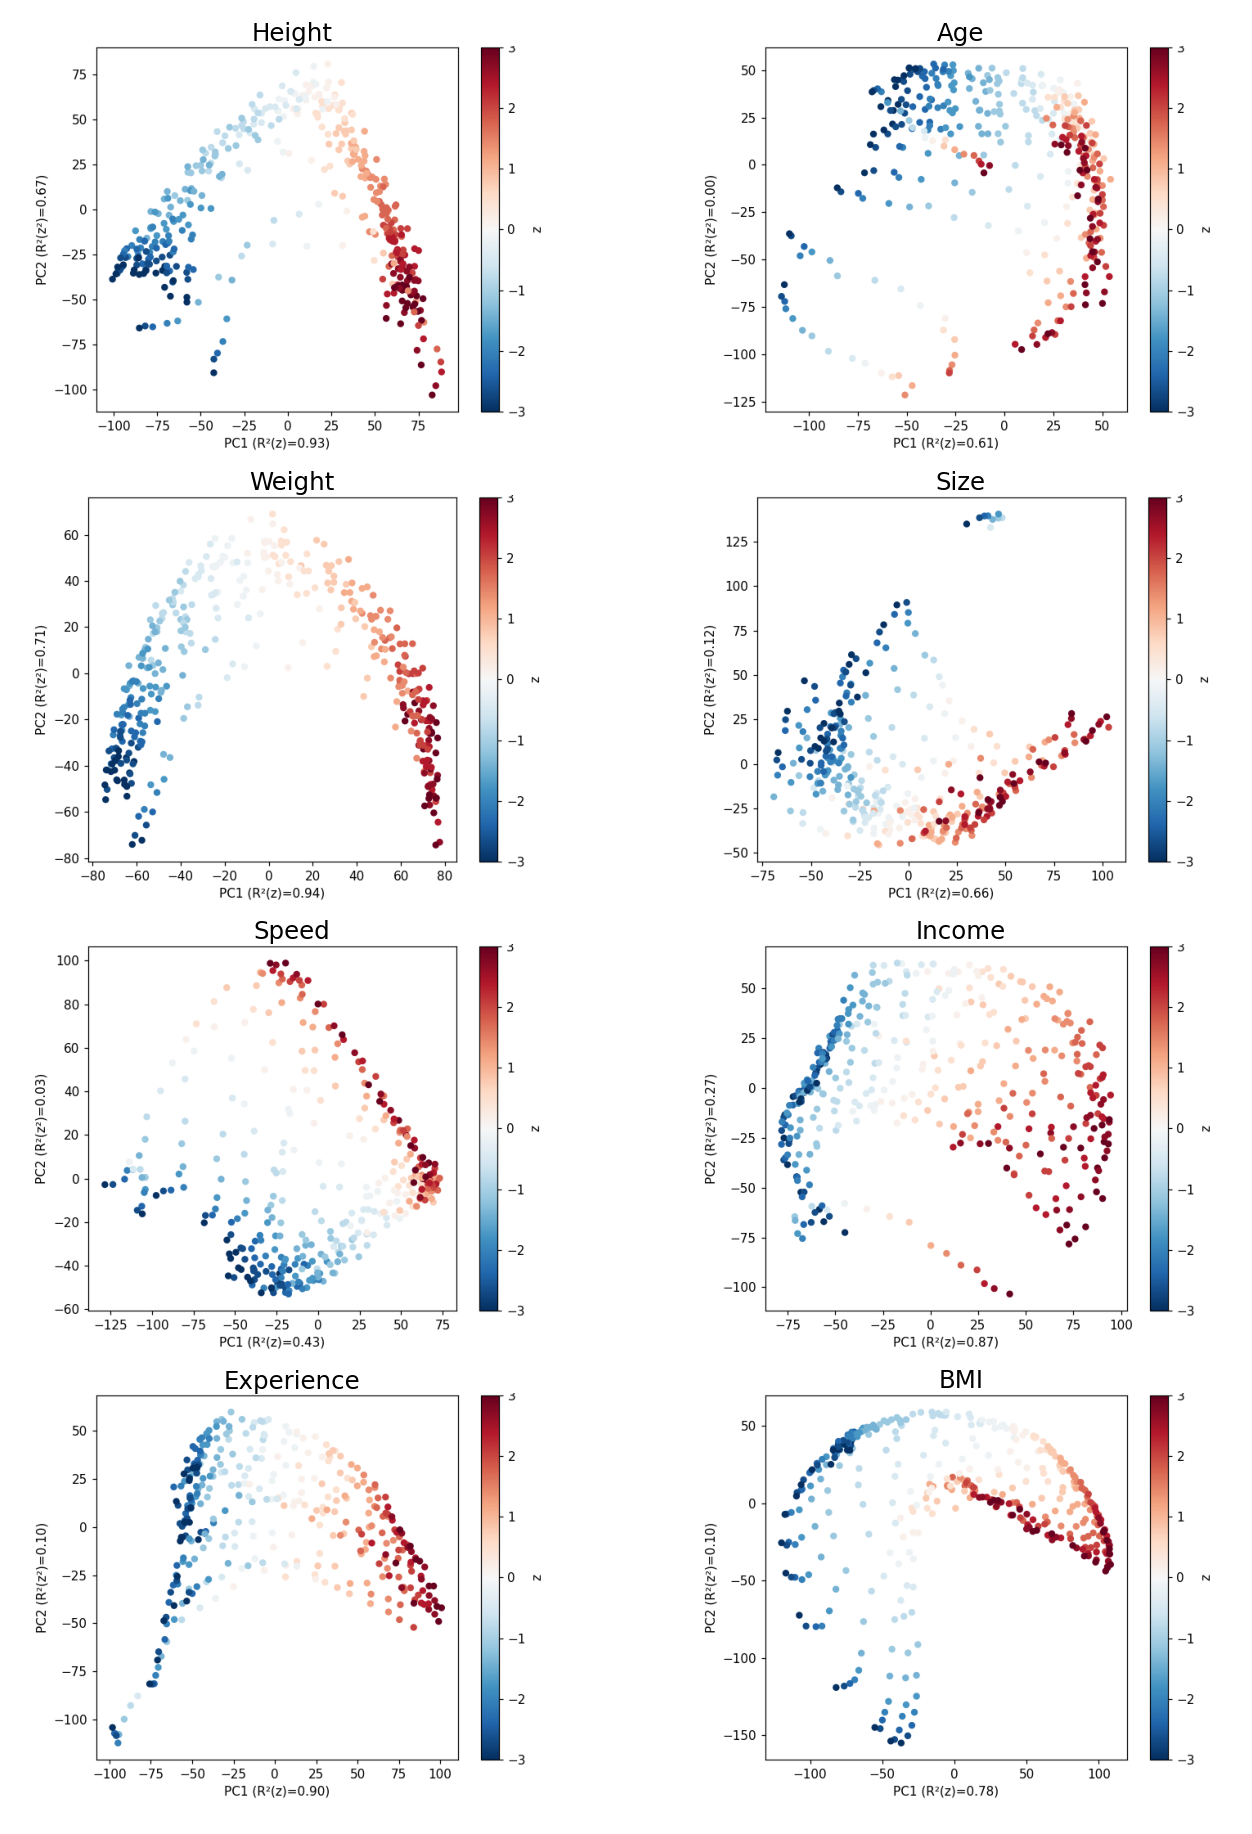
\includegraphics[width=\textwidth,height=0.68\textheight,keepaspectratio]{figures/fig_results_pca_all_pairs_clean.png}
%   \caption{\textbf{Cell-mean activation geometry.}
%   Late-layer PCA views of all eight dense prompt domains show ordered $z$ structure across adjective domains.
%   The plot is geometry evidence, not by itself a mechanism claim.
%   % Source artifacts: figures/v11/pca/*_gemma2-9b_2d_L33.png, cleaned and relabeled for paper display.
%   }
%   \label{fig:pca-montage}
% \end{figure*}


\begin{figure*}[H]
  \centering
  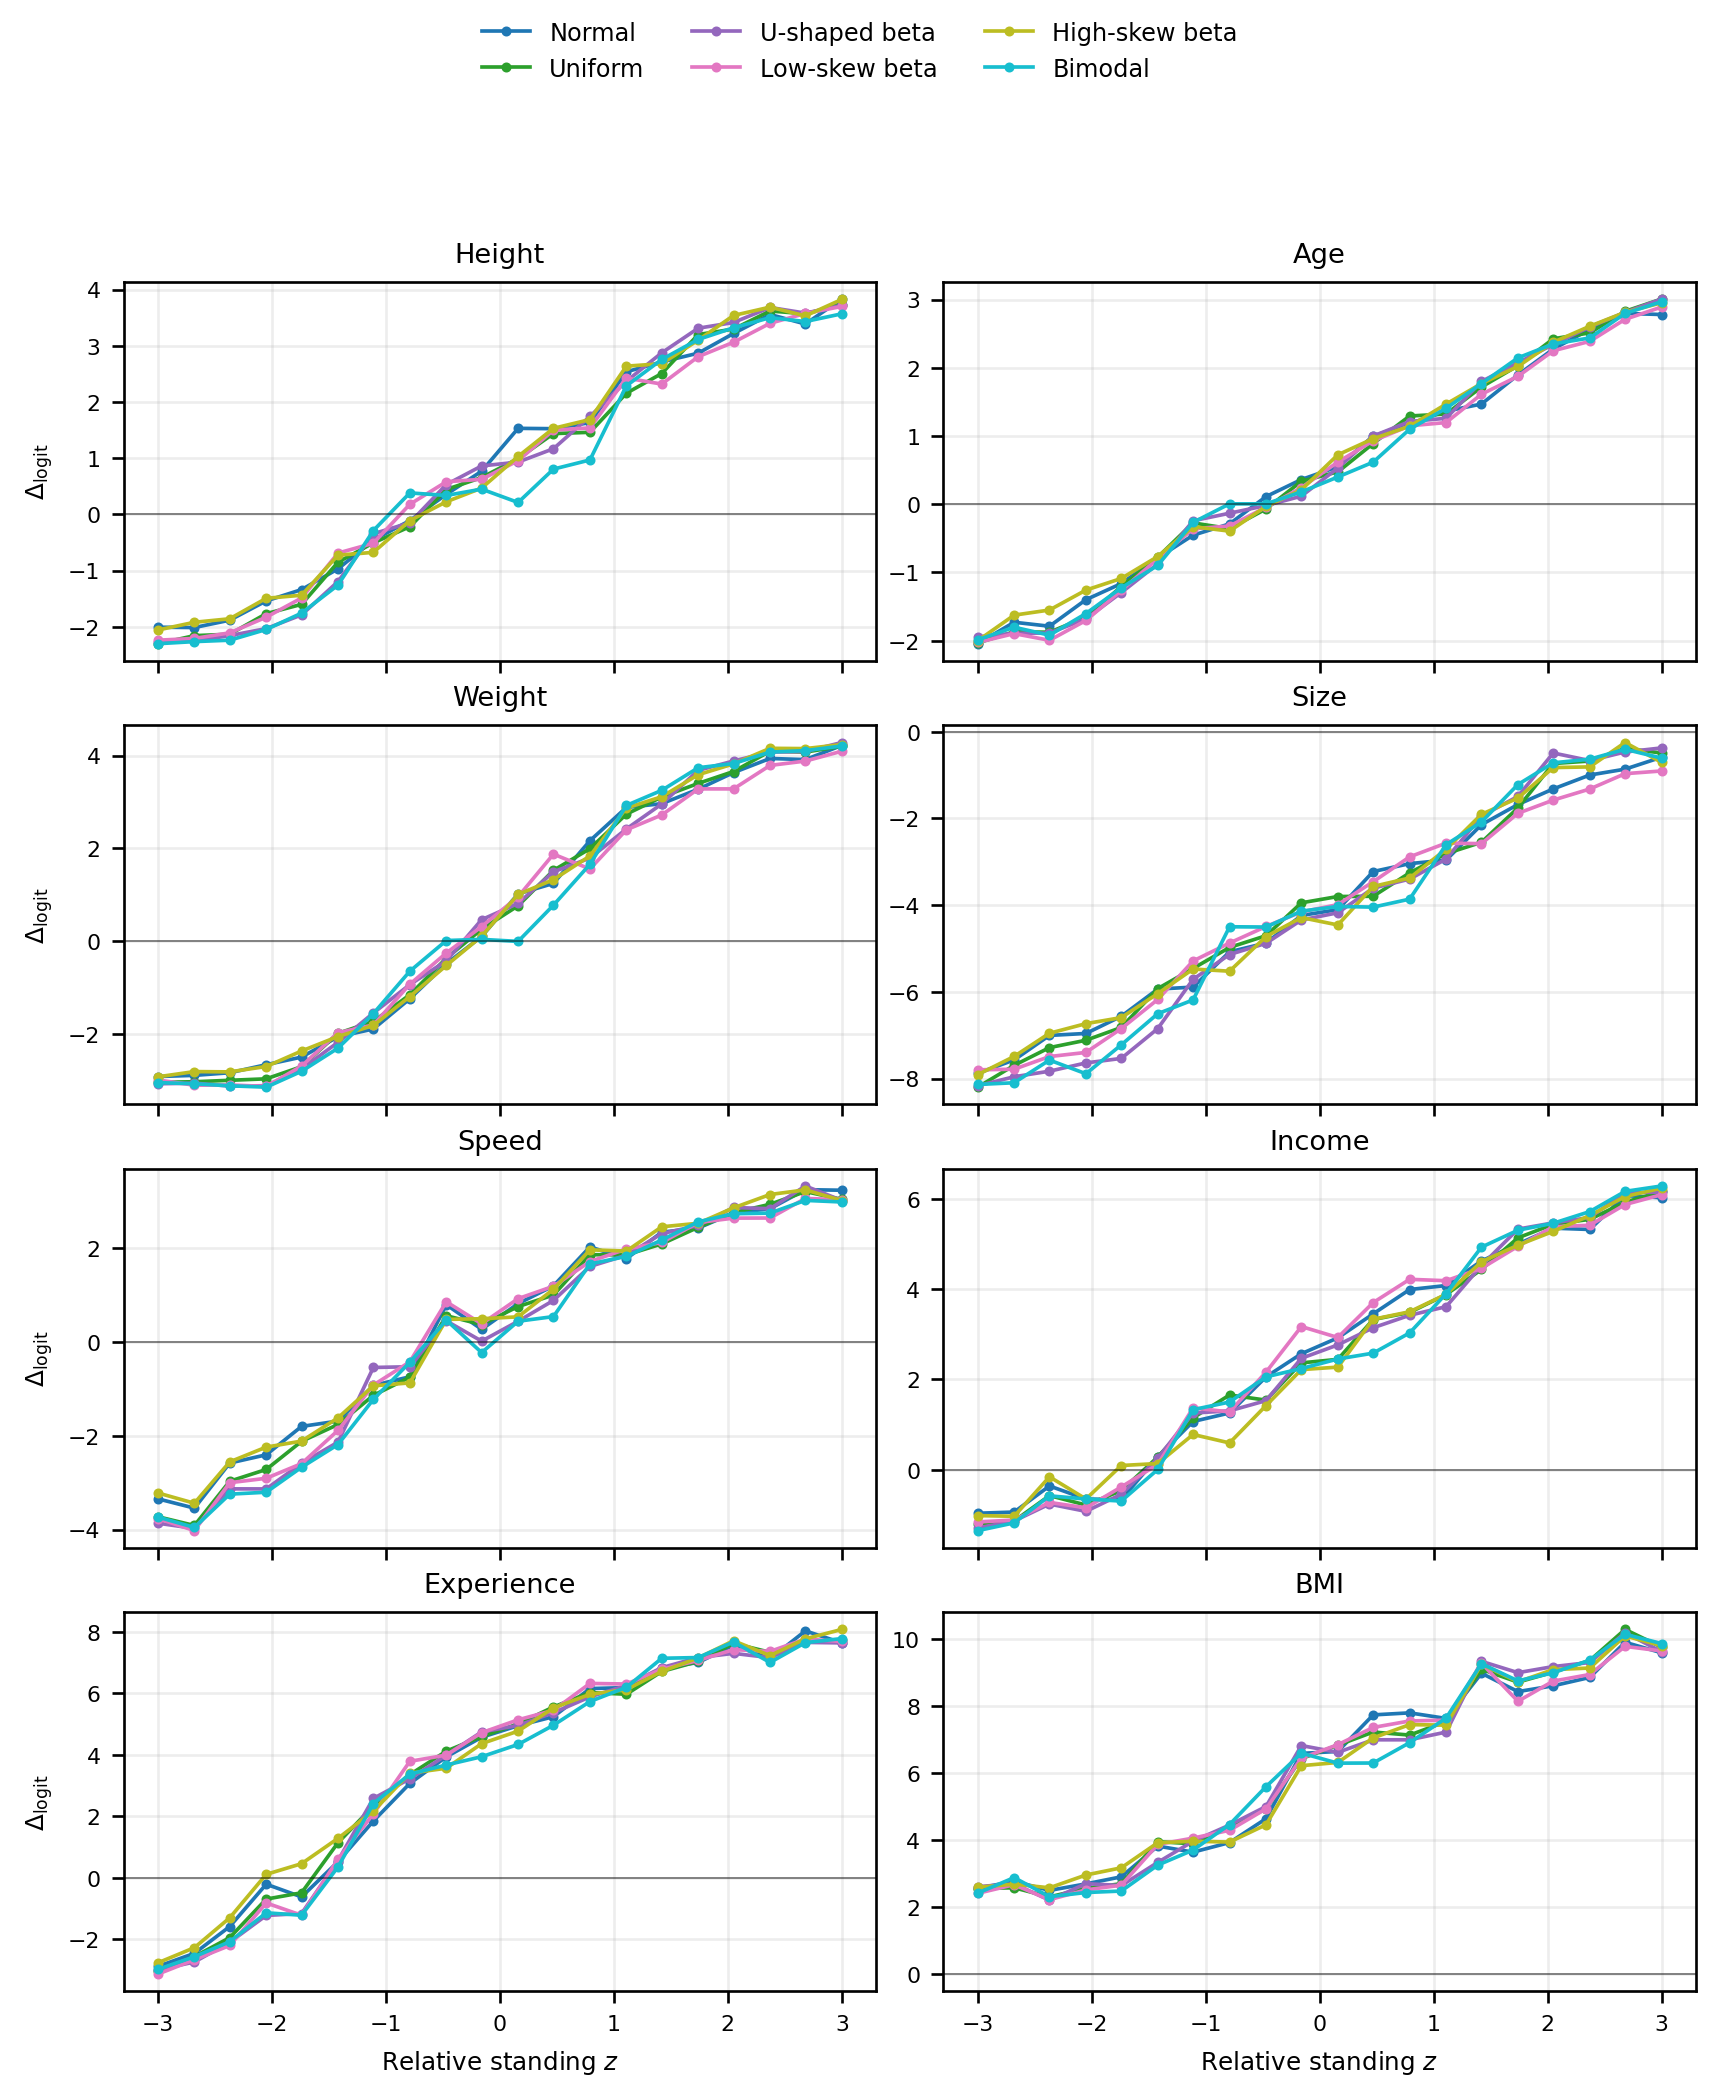
\includegraphics[width=\textwidth,height=0.72\textheight,keepaspectratio]{figures/fig_results_distribution_ld_by_z_clean.png}
  \caption{\textbf{Non-Gaussian context distributions preserve LD-by-$z$ curves.}
  Across normal, uniform, U-shaped, skewed, and bimodal contexts, high-minus-low adjective logit differences remain primarily organized by relative standing.
  % Source artifact: results/v14/distribution/distribution_rows.jsonl, replotted for paper display.
  }
  \label{fig:distribution-robustness-full}
\end{figure*}


\clearpage

% \begin{figure*}[!tbp]
%   \centering
%   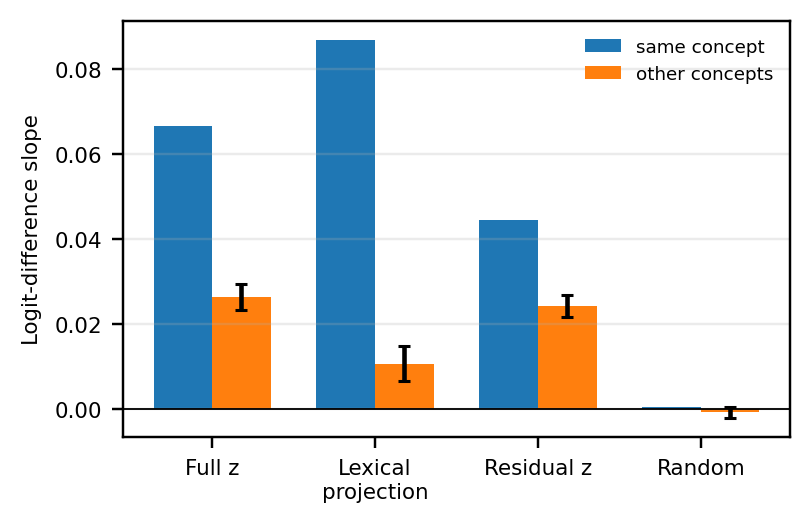
\includegraphics[width=0.5\linewidth]{figures/fig_results_lexical_transfer_summary_clean.png}
%   \caption{\textbf{Shared transfer is not purely lexical.}
%   Projecting onto a lexical adjective subspace gives strong same-concept steering but weak transfer to other concepts.
%   Removing that lexical projection leaves a residual direction with weaker same-concept steering but relatively stronger cross-concept transfer.
%   % Source artifact: results/v12_2/residual_vs_lexical_transfer_summary.json, replotted for paper display.
%   }
%   \label{fig:lexical-residual}
% \end{figure*}

\begin{figure*}[t]
  \centering
  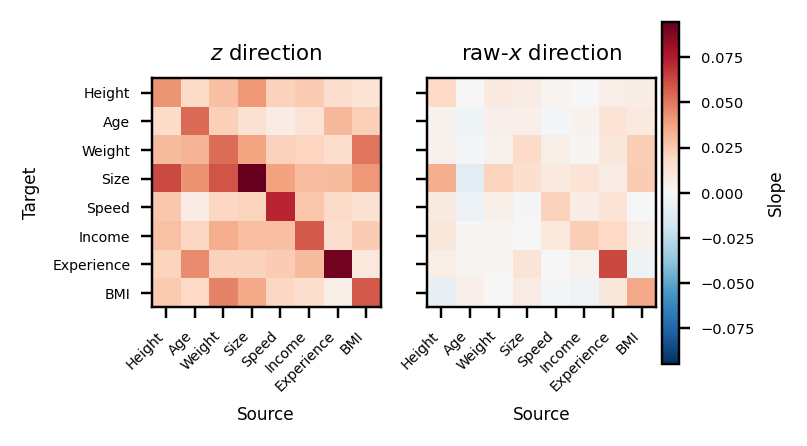
\includegraphics[width=0.82\linewidth]{figures/fig_results_z_vs_x_transfer_clean.png}
  \caption{\textbf{Cross-pair steering transfers more strongly for relative standing than for raw magnitude.}
  Rows are target concepts and columns are source directions.
  Steering with \primalz{} directions produces broadly positive off-diagonal transfer, whereas raw-$x$ directions are much weaker and more diagonal.
  % Source artifacts: results/v13/x_transfer/cross_pair_transfer_x_8x8.json and results/v13/x_transfer/cross_pair_transfer_x_vs_z_summary.json, replotted for paper display.
  }
  \label{fig:z-vs-x-transfer}
\end{figure*}

\begin{figure}[t]
  \centering
  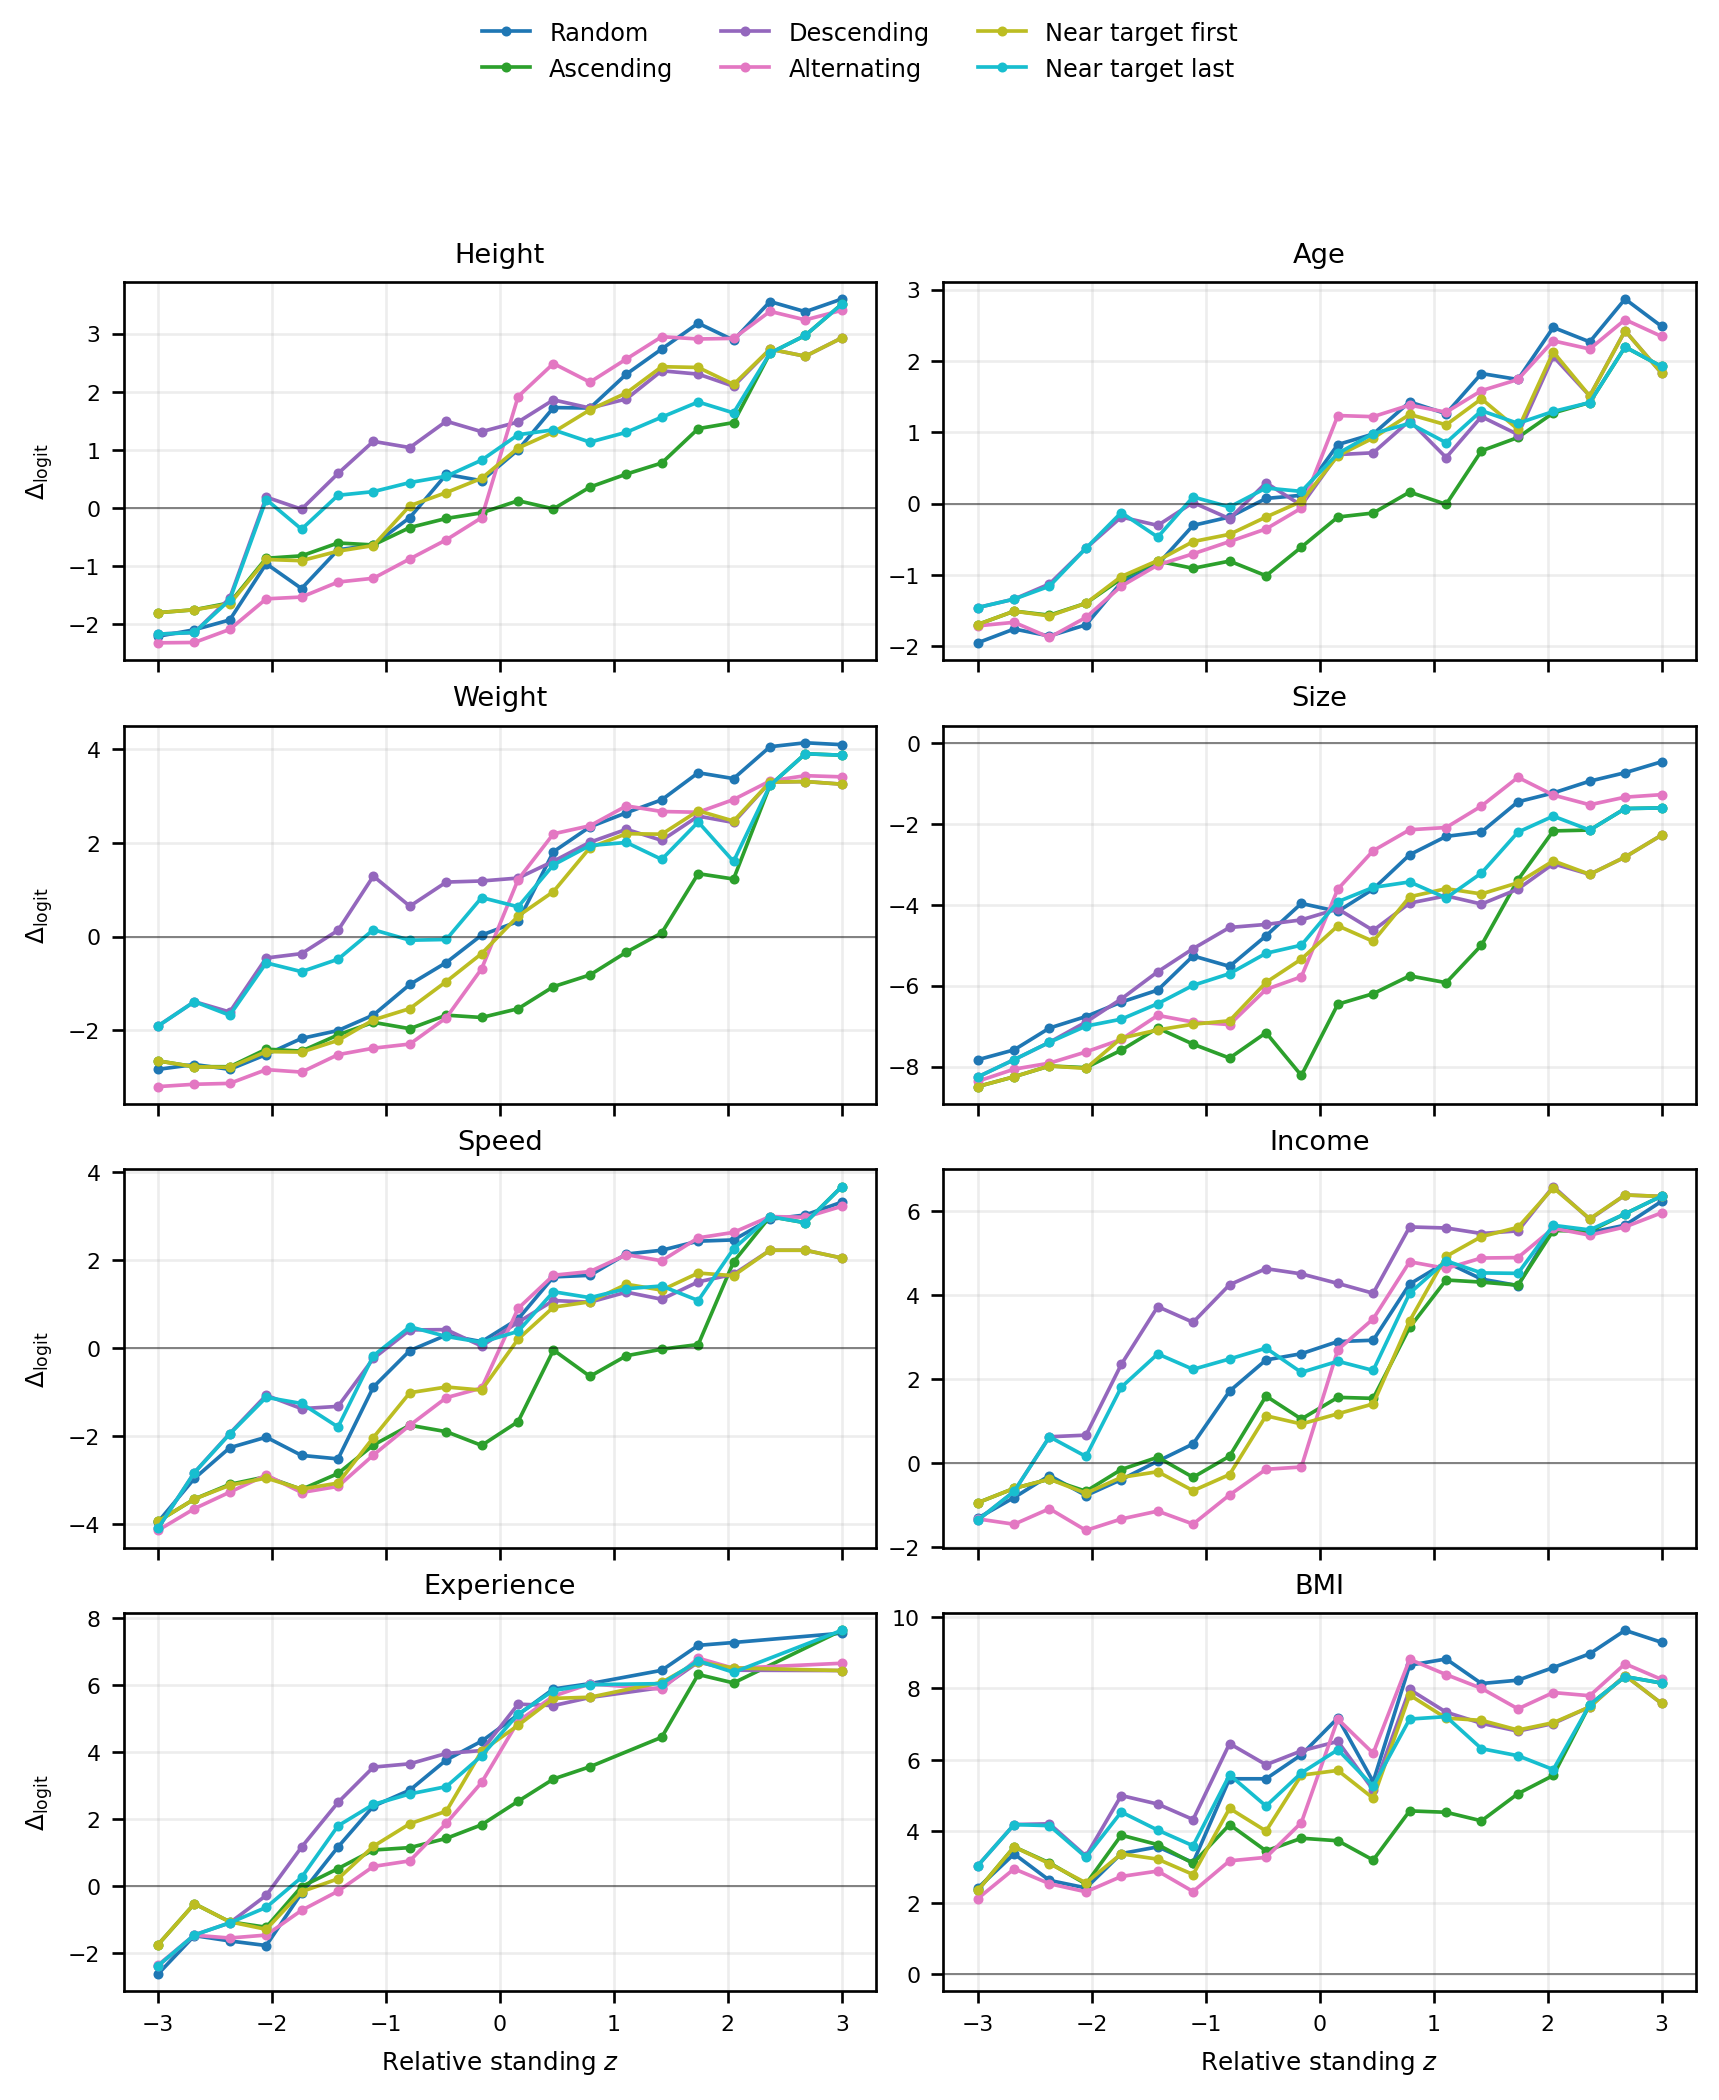
\includegraphics[width=\linewidth]{figures/fig_results_order_ld_by_z_clean.png}
  \caption{\textbf{Context ordering changes affect level and smoothness but do not erase the relative-standing readout.}
  The random order is generally the cleanest baseline, but ascending, descending, alternating, and near-target orderings still preserve a strong monotone LD-by-$z$ relationship.
  % Source artifact: results/v14_1/order/order_rows.jsonl, replotted for paper display.
  }
  \label{fig:order-robustness-full}
\end{figure}


\begin{figure*}[!tbp]
  \centering
  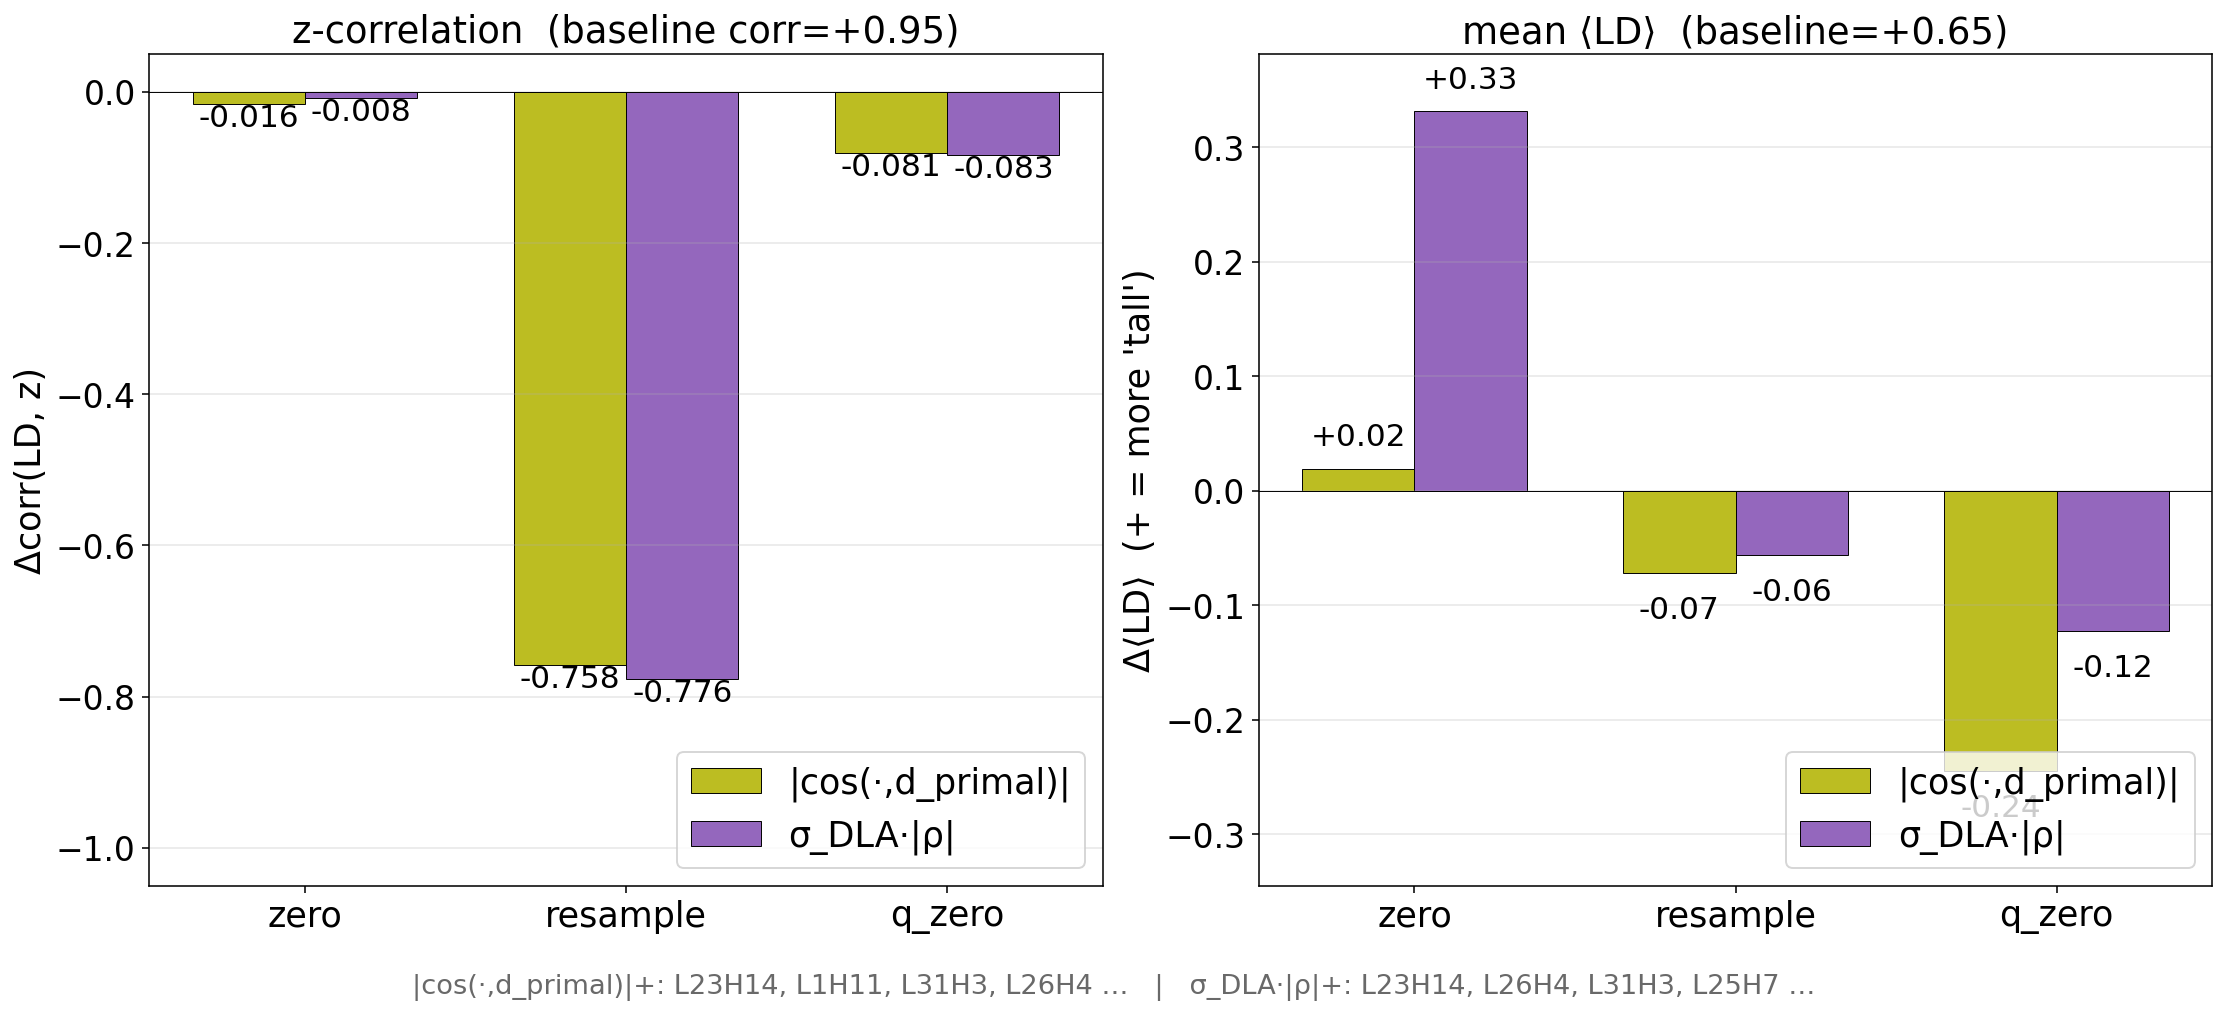
\includegraphics[width=\linewidth]{figures/p2o_attention_modes_comparison_gemma2-9b.png}
  \caption{\textbf{Intervention mode comparison on Gemma-2-9B (height, joint $8$-cell intervention).}
  Left: change in $r(\mathrm{LD},z)$ under three modes --- zero-ablation, resample, and query-zero --- for $8$-head selections by $|\mathrm{cos}|$ and $\sigma_{\mathrm{DLA}}\cdot|\rho|$ methods.
  Right: mean readout shift $\Delta\langle\mathrm{LD}\rangle$ (positive $=$ more ``tall'').
  Zero-ablation barely moves $z$-correlation but pushes the mean readout strongly; resample drains $z$-correlation while leaving the mean readout essentially unchanged.
  Resample is therefore the intervention used throughout this section: it effectively targets relativity.
  % Source artifact: relativity_ablation/figures/p2o_attention_modes_comparison_gemma2-2b.png.
  }
  \label{fig:intervention-modes}
\end{figure*}

\begin{figure*}[!tbp]
  \centering
  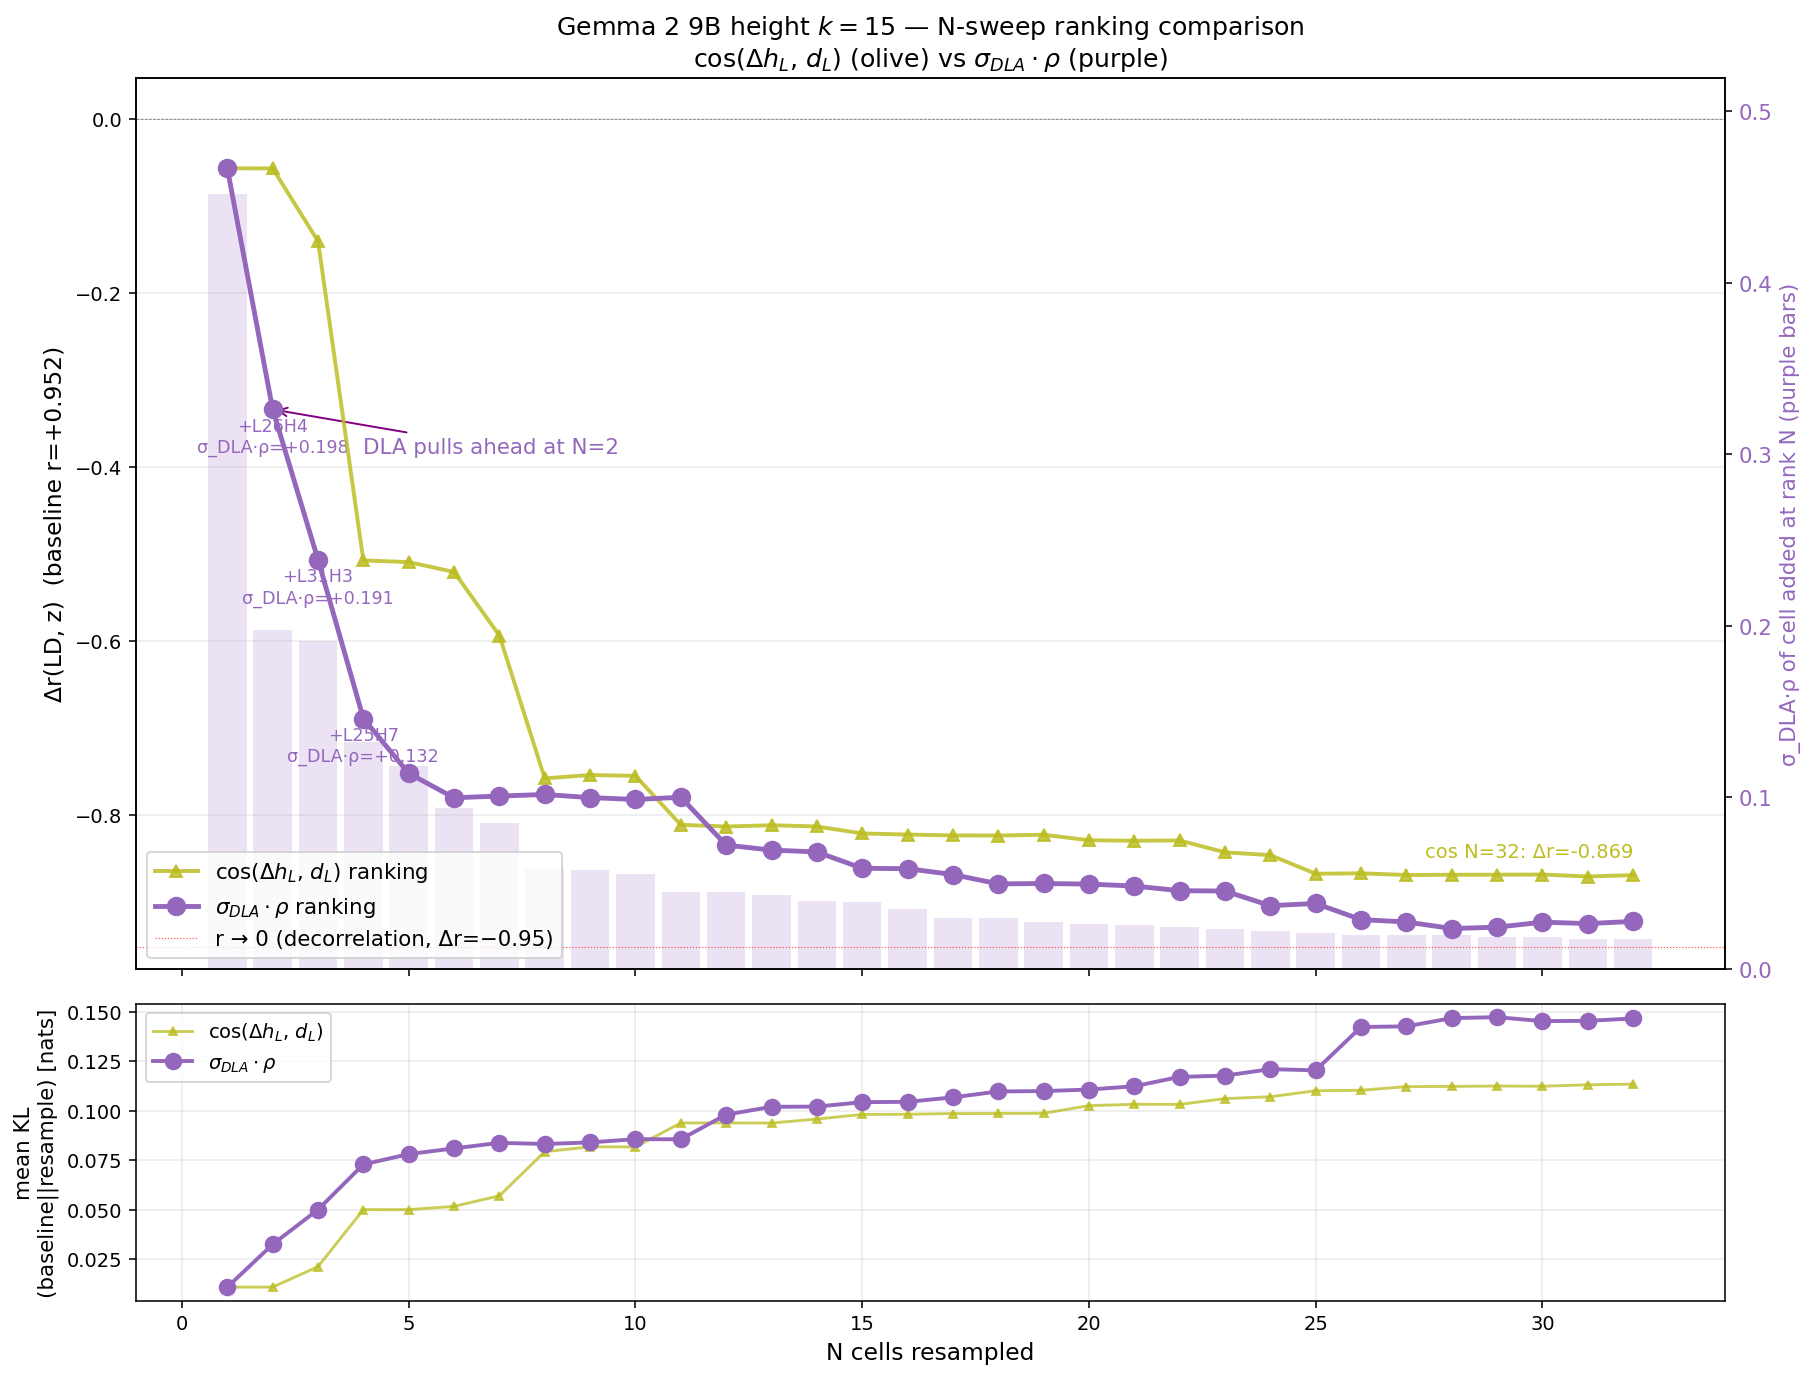
\includegraphics[width=\textwidth,height=0.68\textheight,keepaspectratio]{figures/p2s_dla_vs_cossigma_sweep_gemma2-9b.png}
  \caption{\textbf{Head-ranking comparison on Gemma-2-9B (height, $k{=}15$).}
  Top: $\Delta r(\mathrm{LD}, z)$ under cumulative top-$N$ interchange ablation for the rankings --- $\mathrm{cos}$ and $\sigma_{\mathrm{DLA}}\cdot\rho$ --- with purple bars on the right axis giving the $\sigma_{\mathrm{DLA}}\cdot\rho$ score of the cell entering at rank $N$.
  Bottom: per-prompt mean KL between baseline and resampled next-token distributions for $\mathrm{cos}$ and $\sigma_{\mathrm{DLA}}\cdot\rho$.
  $\sigma_{\mathrm{DLA}}\cdot\rho$ pulls ahead of $\mathrm{cos}$ by $N{=}4$ and at $N{=}8$ already exceeds the $\mathrm{cos}$ saturation ceiling that the latter only approaches at $N{=}32$, ultimately driving the readout to near-decorrelation ($\Delta corr{\approx}{-}0.93$).
  % Source artifact: relativity_ablation/figures/p2s_dla_vs_cossigma_sweep_gemma2-2b.png.
  }
  \label{fig:ranking-comparison}
\end{figure*}

\begin{figure*}[!tbp]
  \centering
  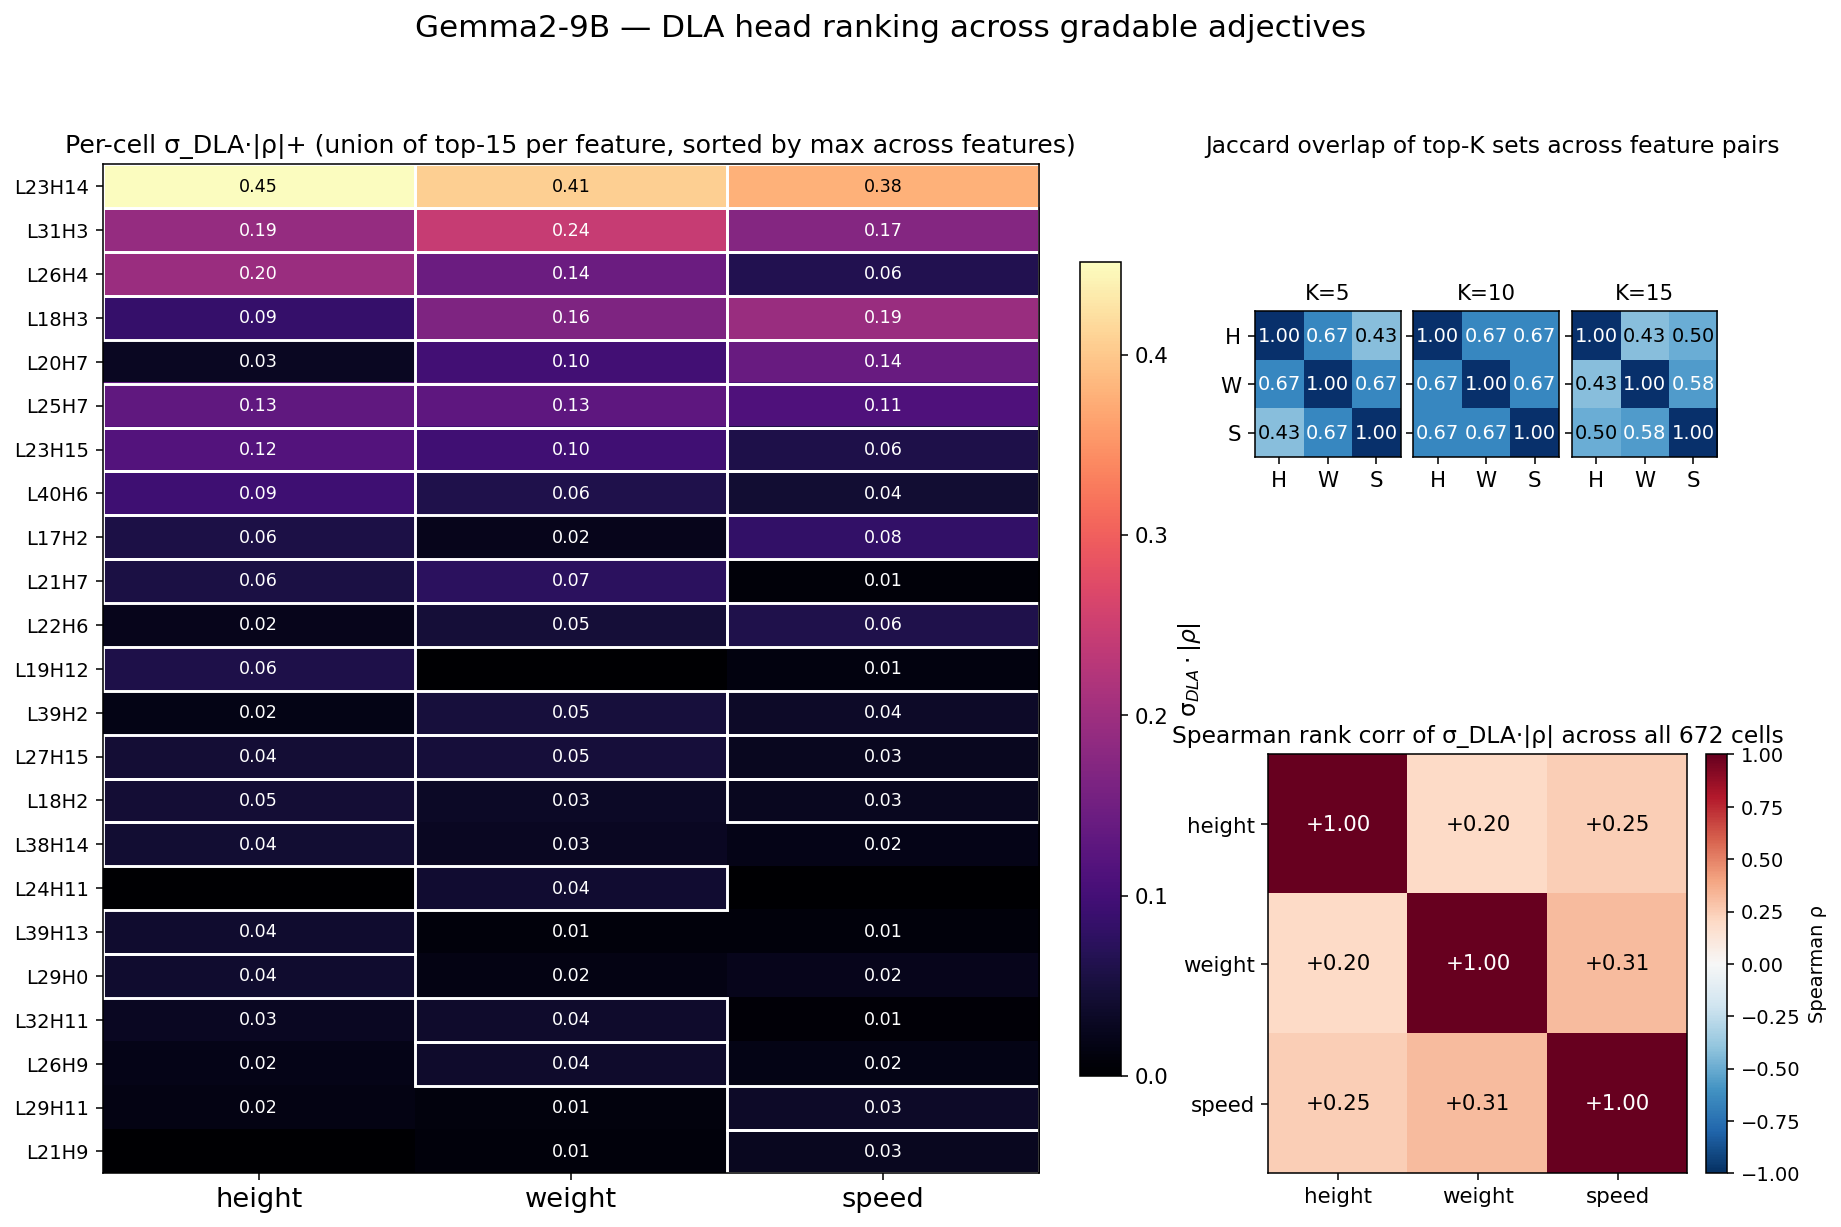
\includegraphics[width=\textwidth,height=0.68\textheight,keepaspectratio]{figures/p2s_dla_xfeat_summary_gemma2-9b.png}
  \caption{\textbf{Heads recovered by various gradable adjectives using DLA}
  We see very strong similarity in heads recovered by using DLA on any of the relativity concepts height, weight and speed.
  % Source artifact: relativity_ablation/figures/p2s_dla_vs_cossigma_sweep_gemma2-2b.png.
  }
  \label{fig:fingerprint}
\end{figure*}

\begin{figure*}[!tbp]
  \centering
  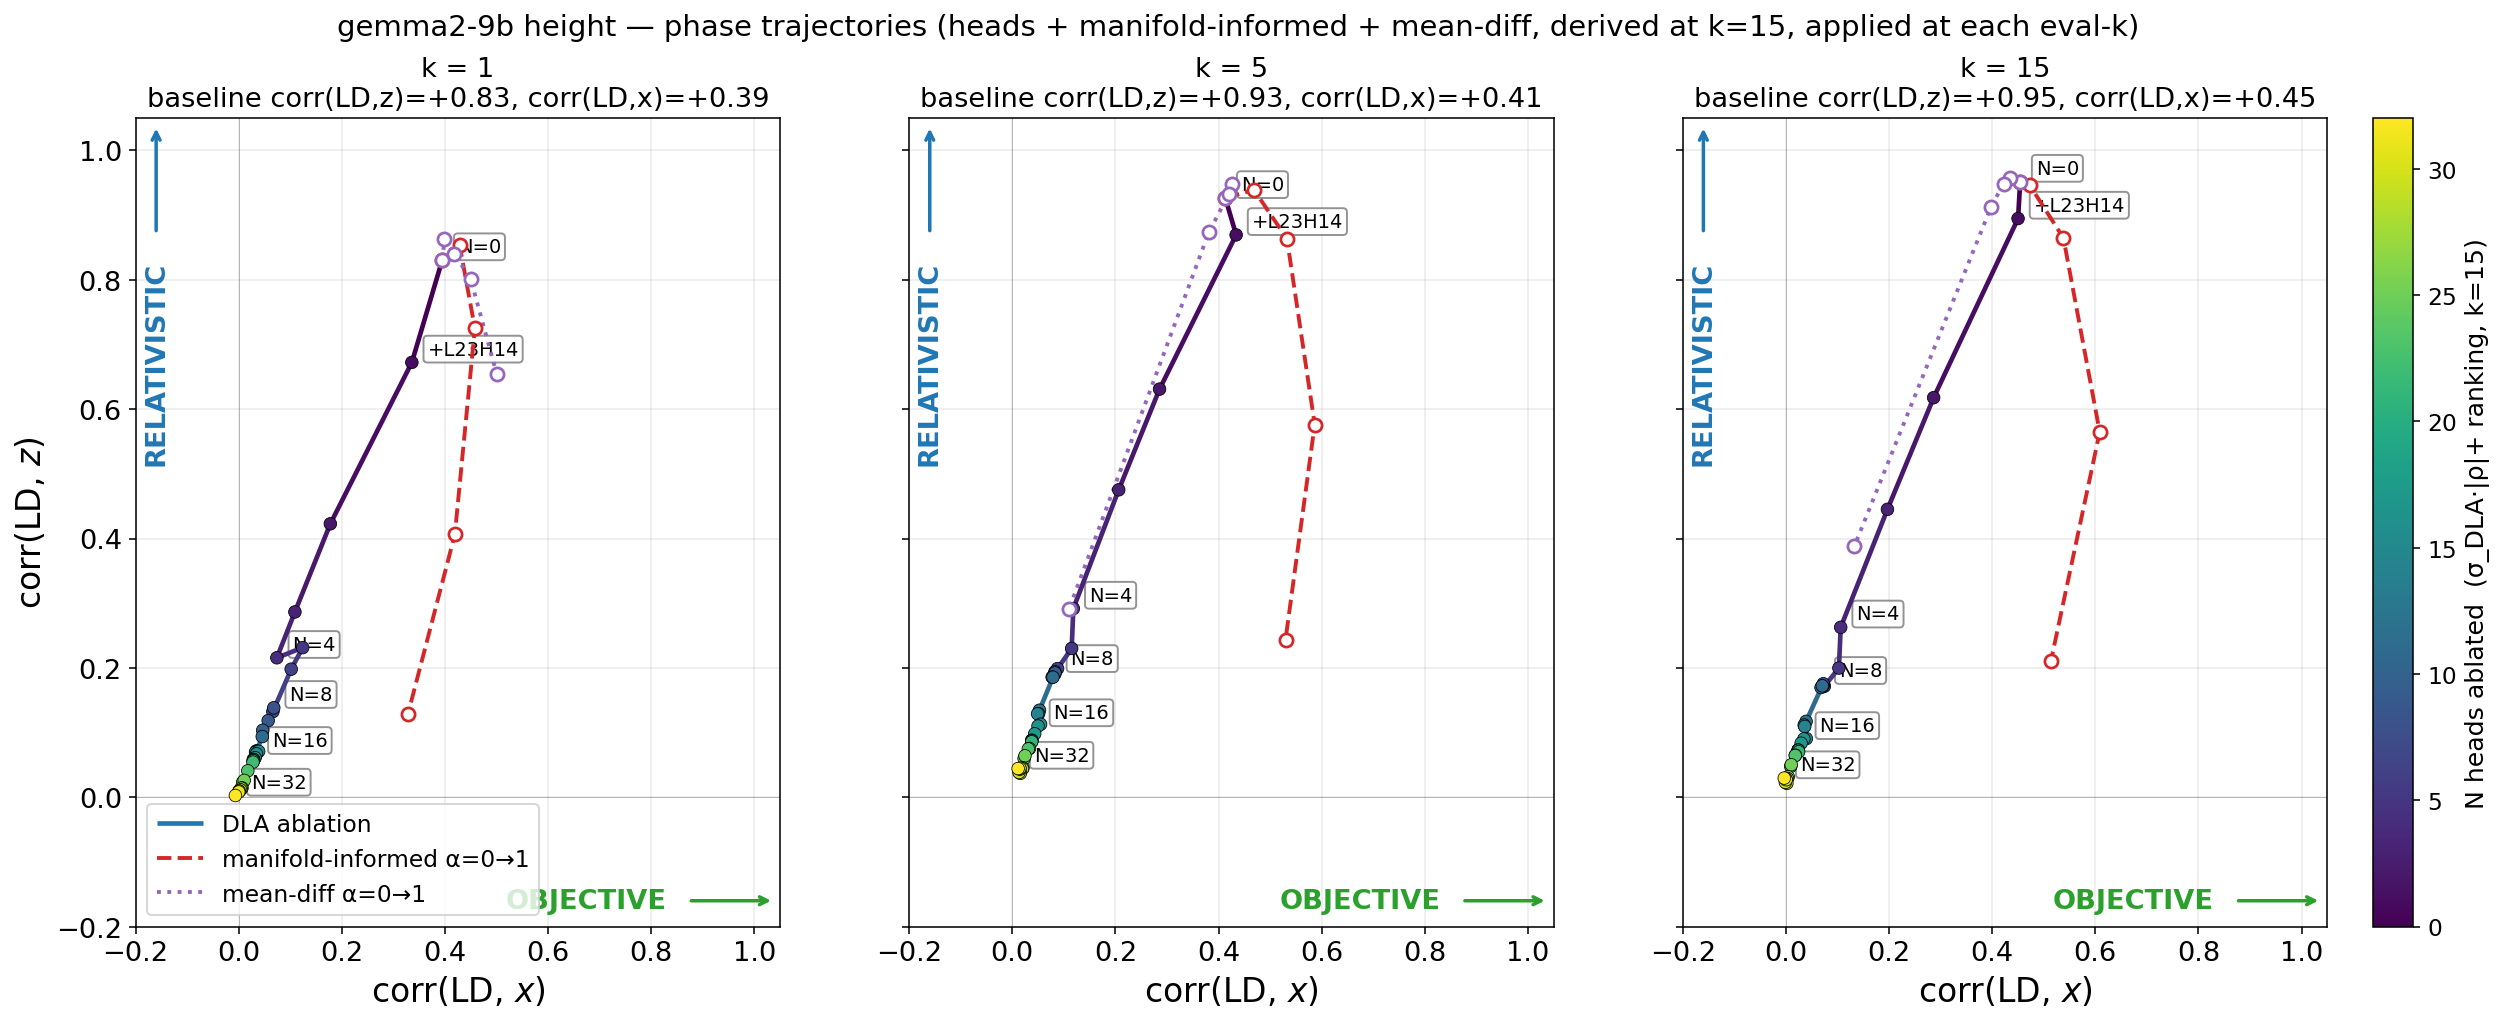
\includegraphics[width=\textwidth,height=0.68\textheight,keepaspectratio]{figures/p2v_xk_corr_grid_gemma2-9b_height.png}
 \caption{\textbf{The same heads, mean-diff direction, and manifold lookup
  collapse the relativity readout at every shot count.}
  Each panel evaluates the $k{=}15$-derived intervention triplet
  (DLA head ranking, mean-diff direction
  $\hat d_L$, and arc-length manifold lookup $M$) on a different stimulus
  distribution ($k{\in}\{1,5,15\}$) on Gemma-2-9B, in the
  $\big(\mathrm{corr}(\mathrm{LD},x),\,\mathrm{corr}(\mathrm{LD},z)\big)$
  phase plane.
  Both attention and mean diff ablation methods destroy objectivity in their process, manifold steering mostly preserves.
  % Source artifact: relativity_ablation/figures/p2v_xk_corr_grid_gemma2-9b_height.png.
  }
  \label{fig:xk-corr-grid-9b-height}
\end{figure*}

\begin{figure*}[!tbp]
  \centering
  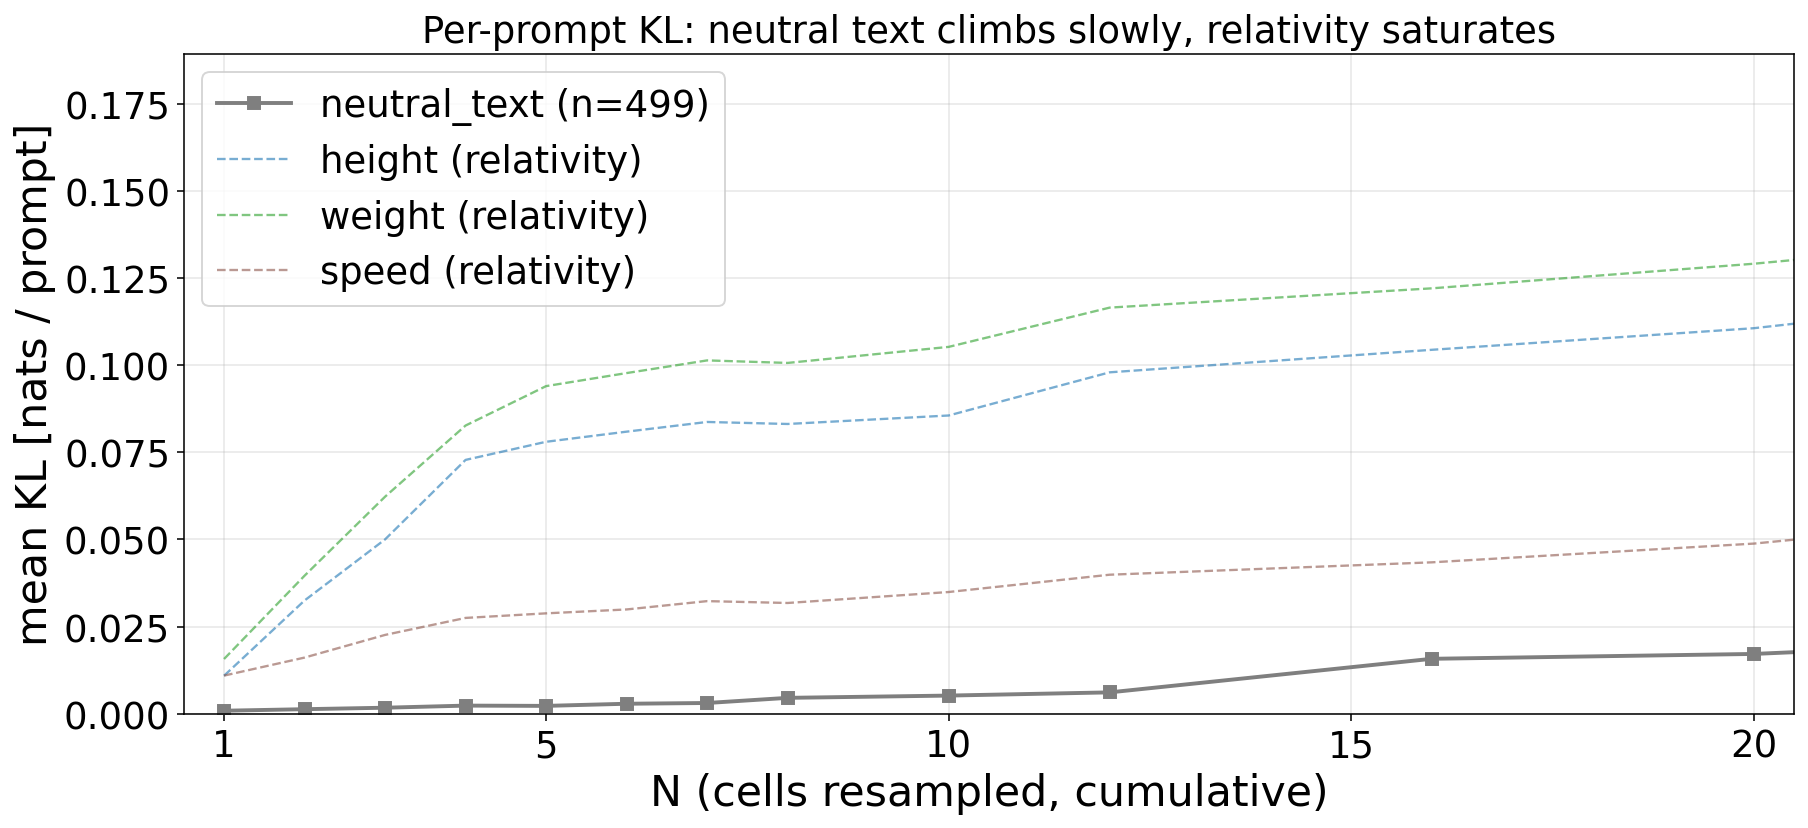
\includegraphics[width=\textwidth,height=0.68\textheight,keepaspectratio]{figures/p2u_n_sweep_xfeat_gemma2-9b_kl.png}
  \caption{\textbf{KL divergence on next token generation under N-head ablation chosen by DLA on height}
  KL divergence barely moves for natural language next token prediction when compared to relativity concepts.
  % Source artifact: relativity_ablation/figures/p2s_dla_vs_cossigma_sweep_gemma2-2b.png.
  }
  \label{fig:kl}
\end{figure*}

\begin{figure*}[!tbp]
  \centering
  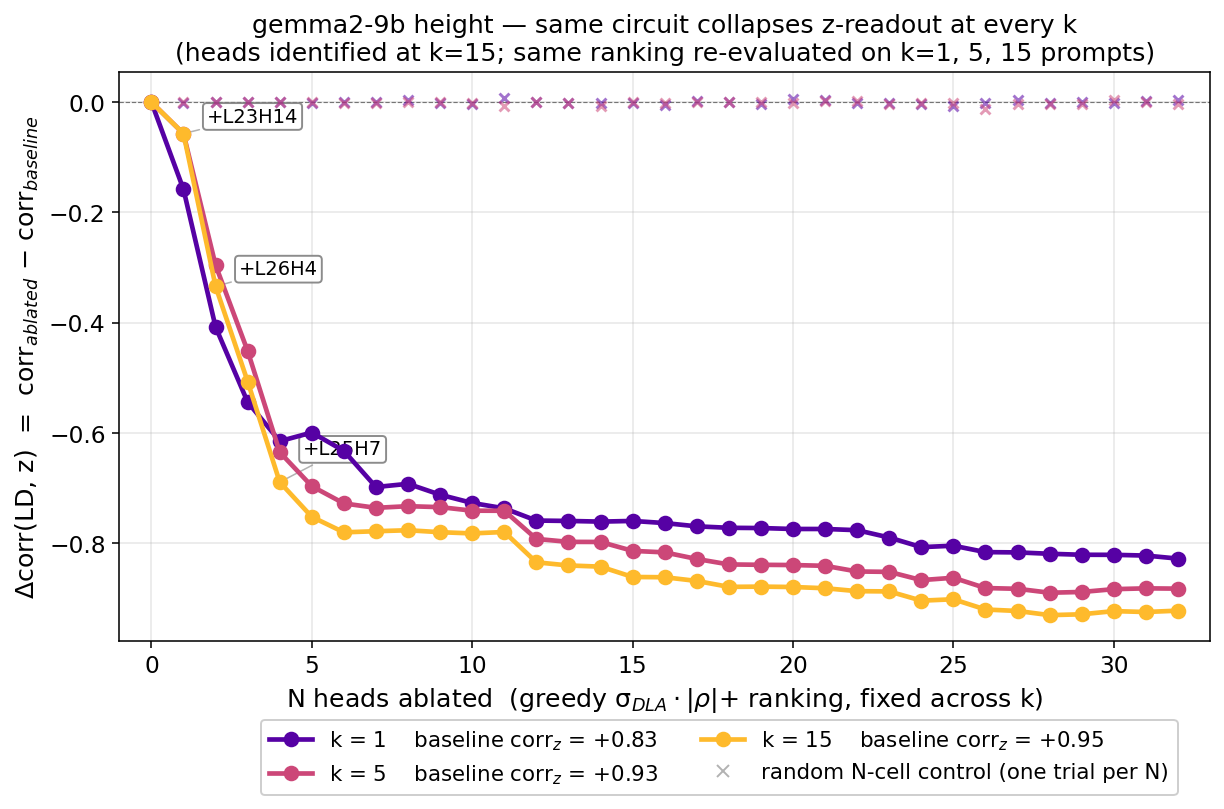
\includegraphics[width=\textwidth,height=0.68\textheight,keepaspectratio]{figures/p2v_xk_deltar_overlay_gemma2-9b_height.png}
  \caption{\textbf{Greedy resample under a fixed head ranking is
  $k$-invariant.}
  $\Delta\mathrm{corr}(\mathrm{LD}, z)$ vs $N$ on Gemma-2-9B for the same
  $\sigma_{\mathrm{DLA}}\cdot|\rho|$+ ranking (derived once at $k{=}15$,
  then re-applied at $k{\in}\{1, 5, 15\}$).
  All three curves descend monotonically and saturate at
  $\Delta\mathrm{corr}{=}{-}0.83$ ($k{=}1$, baseline $+0.83$),
  ${-}0.88$ ($k{=}5$, baseline $+0.93$), and
  ${-}0.92$ ($k{=}15$, baseline $+0.95$).
  Random $N$-cell controls ($\times$) hover near zero.
  % Source artifact: relativity_ablation/figures/p2v_xk_deltar_overlay_gemma2-9b_height.png.
  }
  \label{fig:xk-deltar-overlay-9b-height}
\end{figure*}


\begin{figure*}[!tbp]
  \centering
  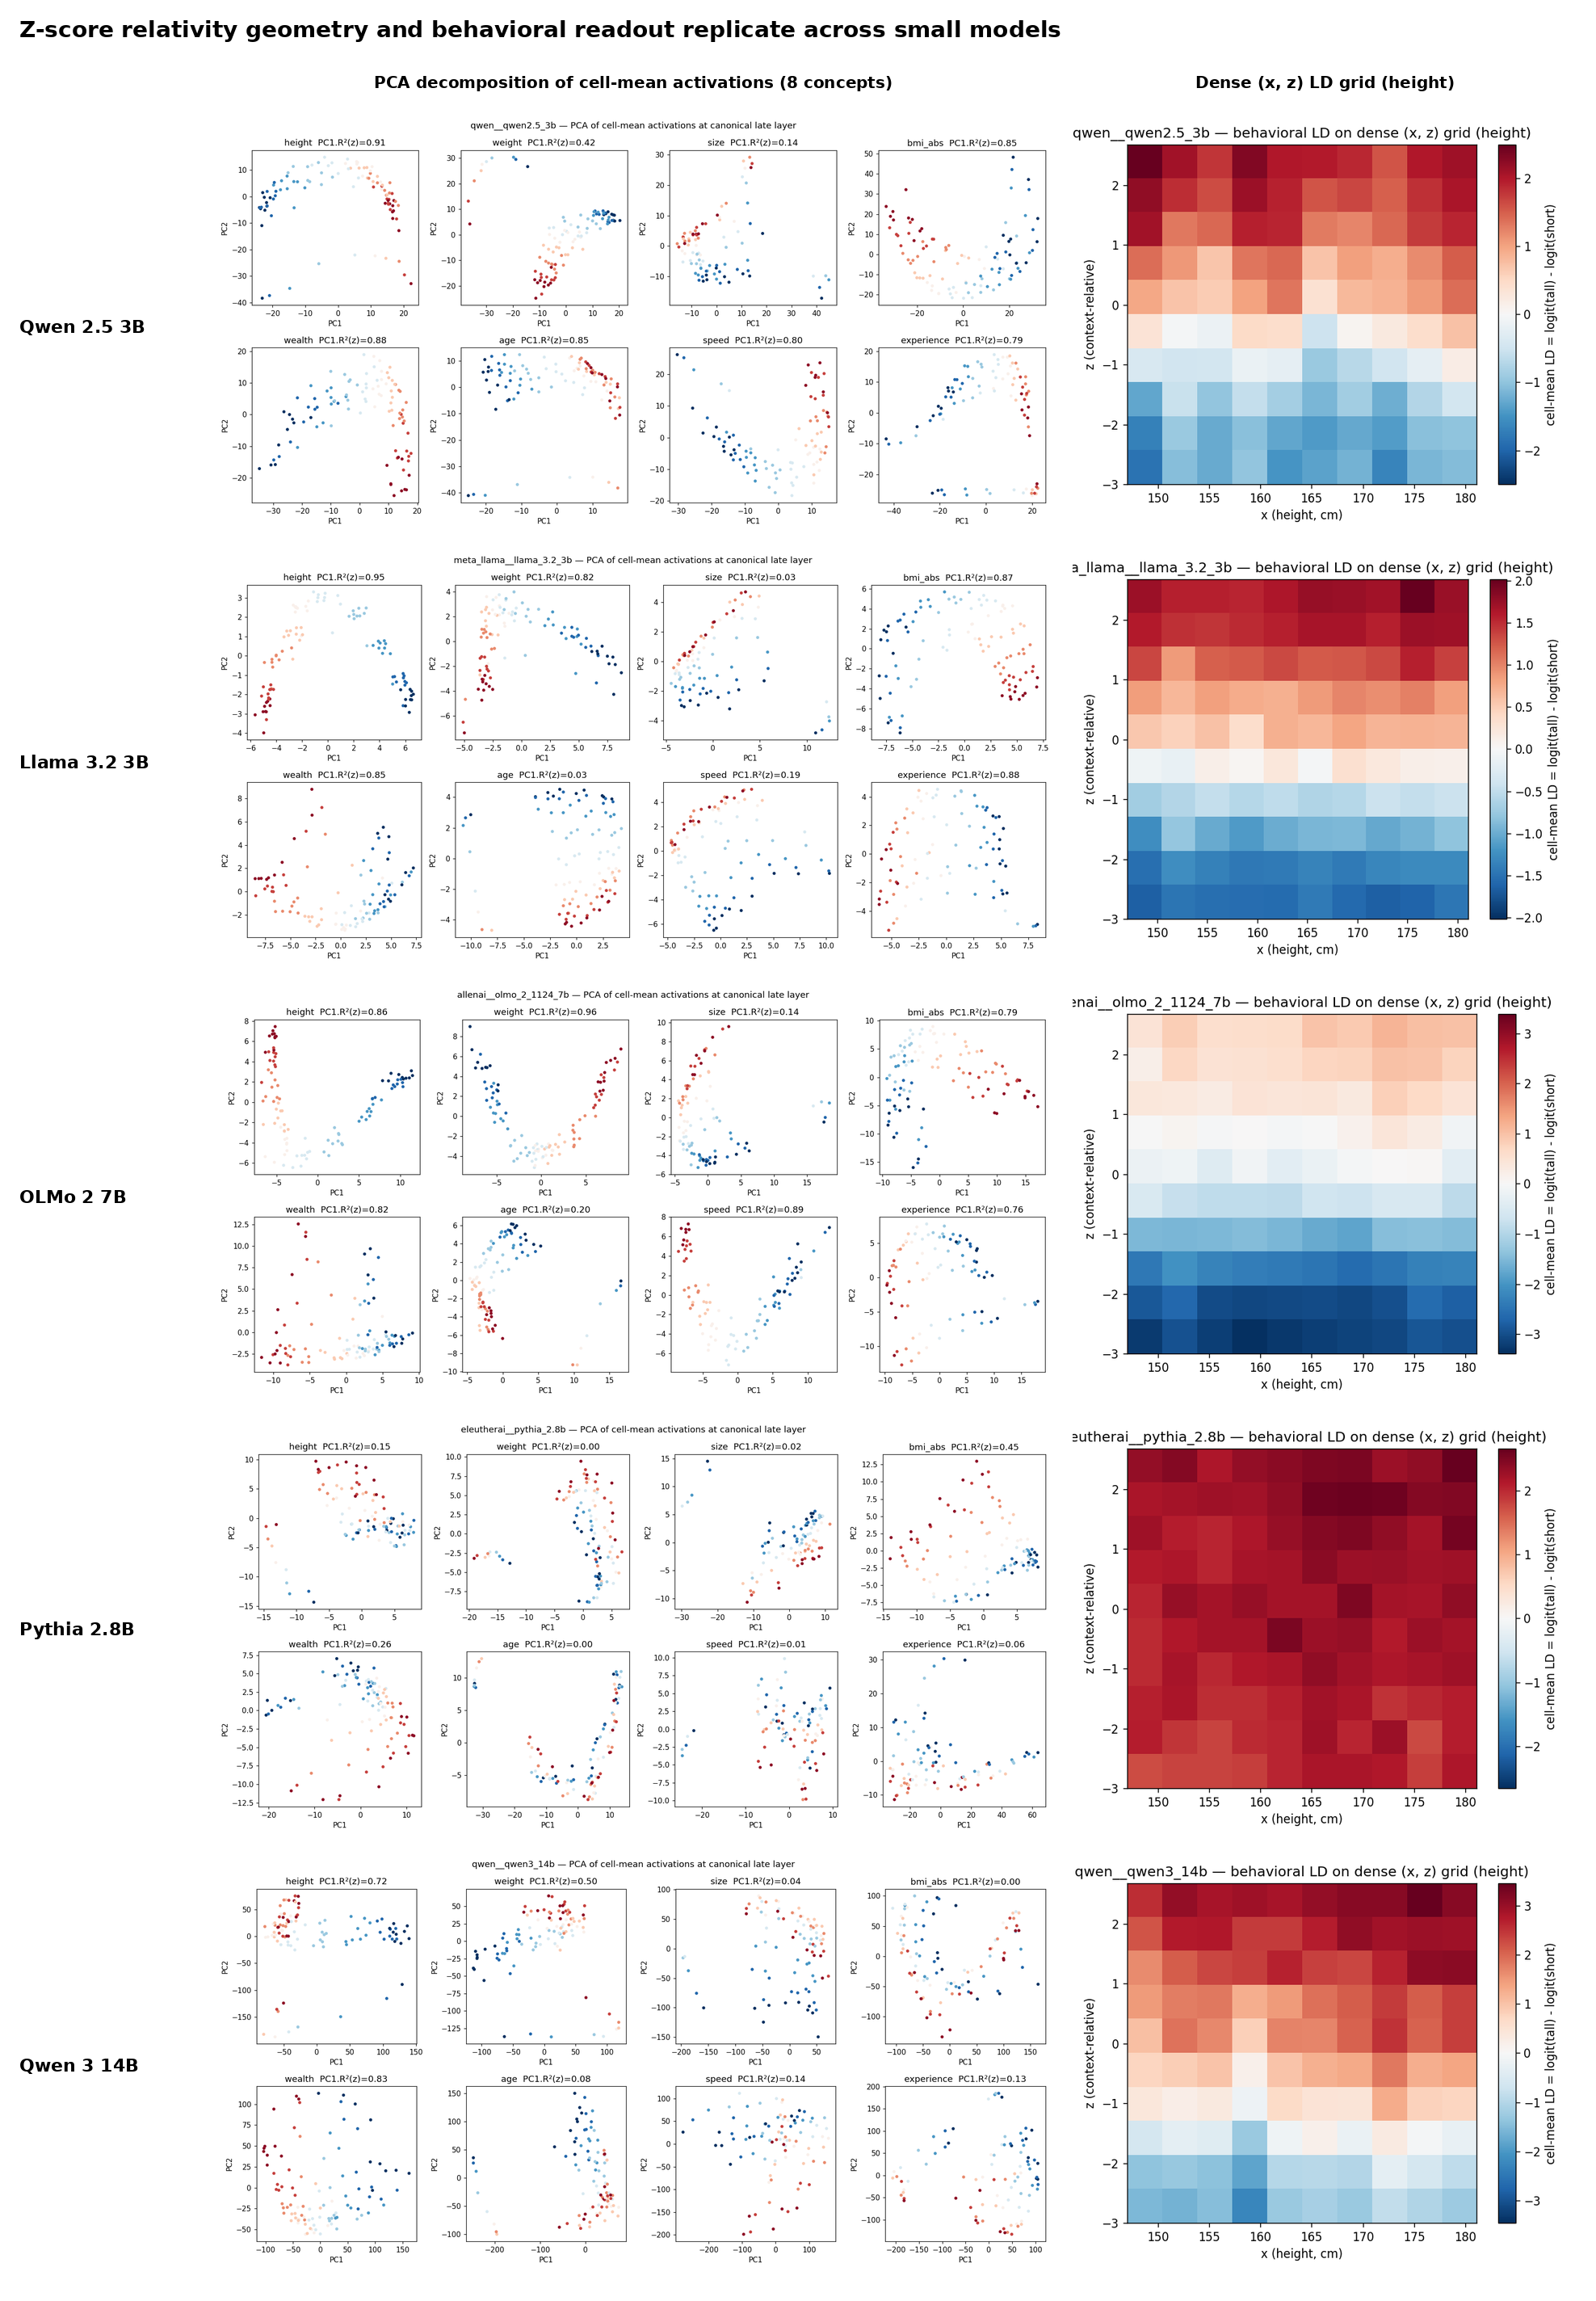
\includegraphics[width=0.8\linewidth]{figures/xmodel_geometry_grid.png}
  \caption{\textbf{Z-score relativity geometry and dense-grid behavior
  replicate across five small open-weights models.}
  Rows: Qwen 2.5 3B, Llama 3.2 3B, OLMo 2 7B, Pythia 2.8B, Qwen 3 14B.
  Left column: PCA decomposition of cell-mean activations at each model's
  canonical late layer, one panel per concept (height, weight, size, bmi,
  wealth, age, speed, experience). Each panel reports
  $R^2(z\mid\mathrm{PC1})$; values $\geq 0.7$ on graded concepts indicate
  that the leading principal component of the cell-mean activation tracks
  the context-relative $z$-score rather than the raw value.
  Right column: behavioral $\mathrm{LD}=\mathrm{logit}(\text{tall})-\mathrm{logit}(\text{short})$
  on the dense $(x, z)$ grid for the height pair.
  Four of the five models show the same vertical-stripe pattern --- $\mathrm{LD}$
  varies primarily with $z$ and only weakly with $x$ --- consistent with the
  Gemma 2 result in the main text. Pythia 2.8B is the only exception.
  % Source: relativity_ablation/scripts/p2v_xmodel_appendix_composites.py;
  %         per-model panels under geometry-of-relativity/figures/v13/.
  }
  \label{fig:xmodel-geometry}
\end{figure*}


\begin{figure*}[!tbp]
  \centering
  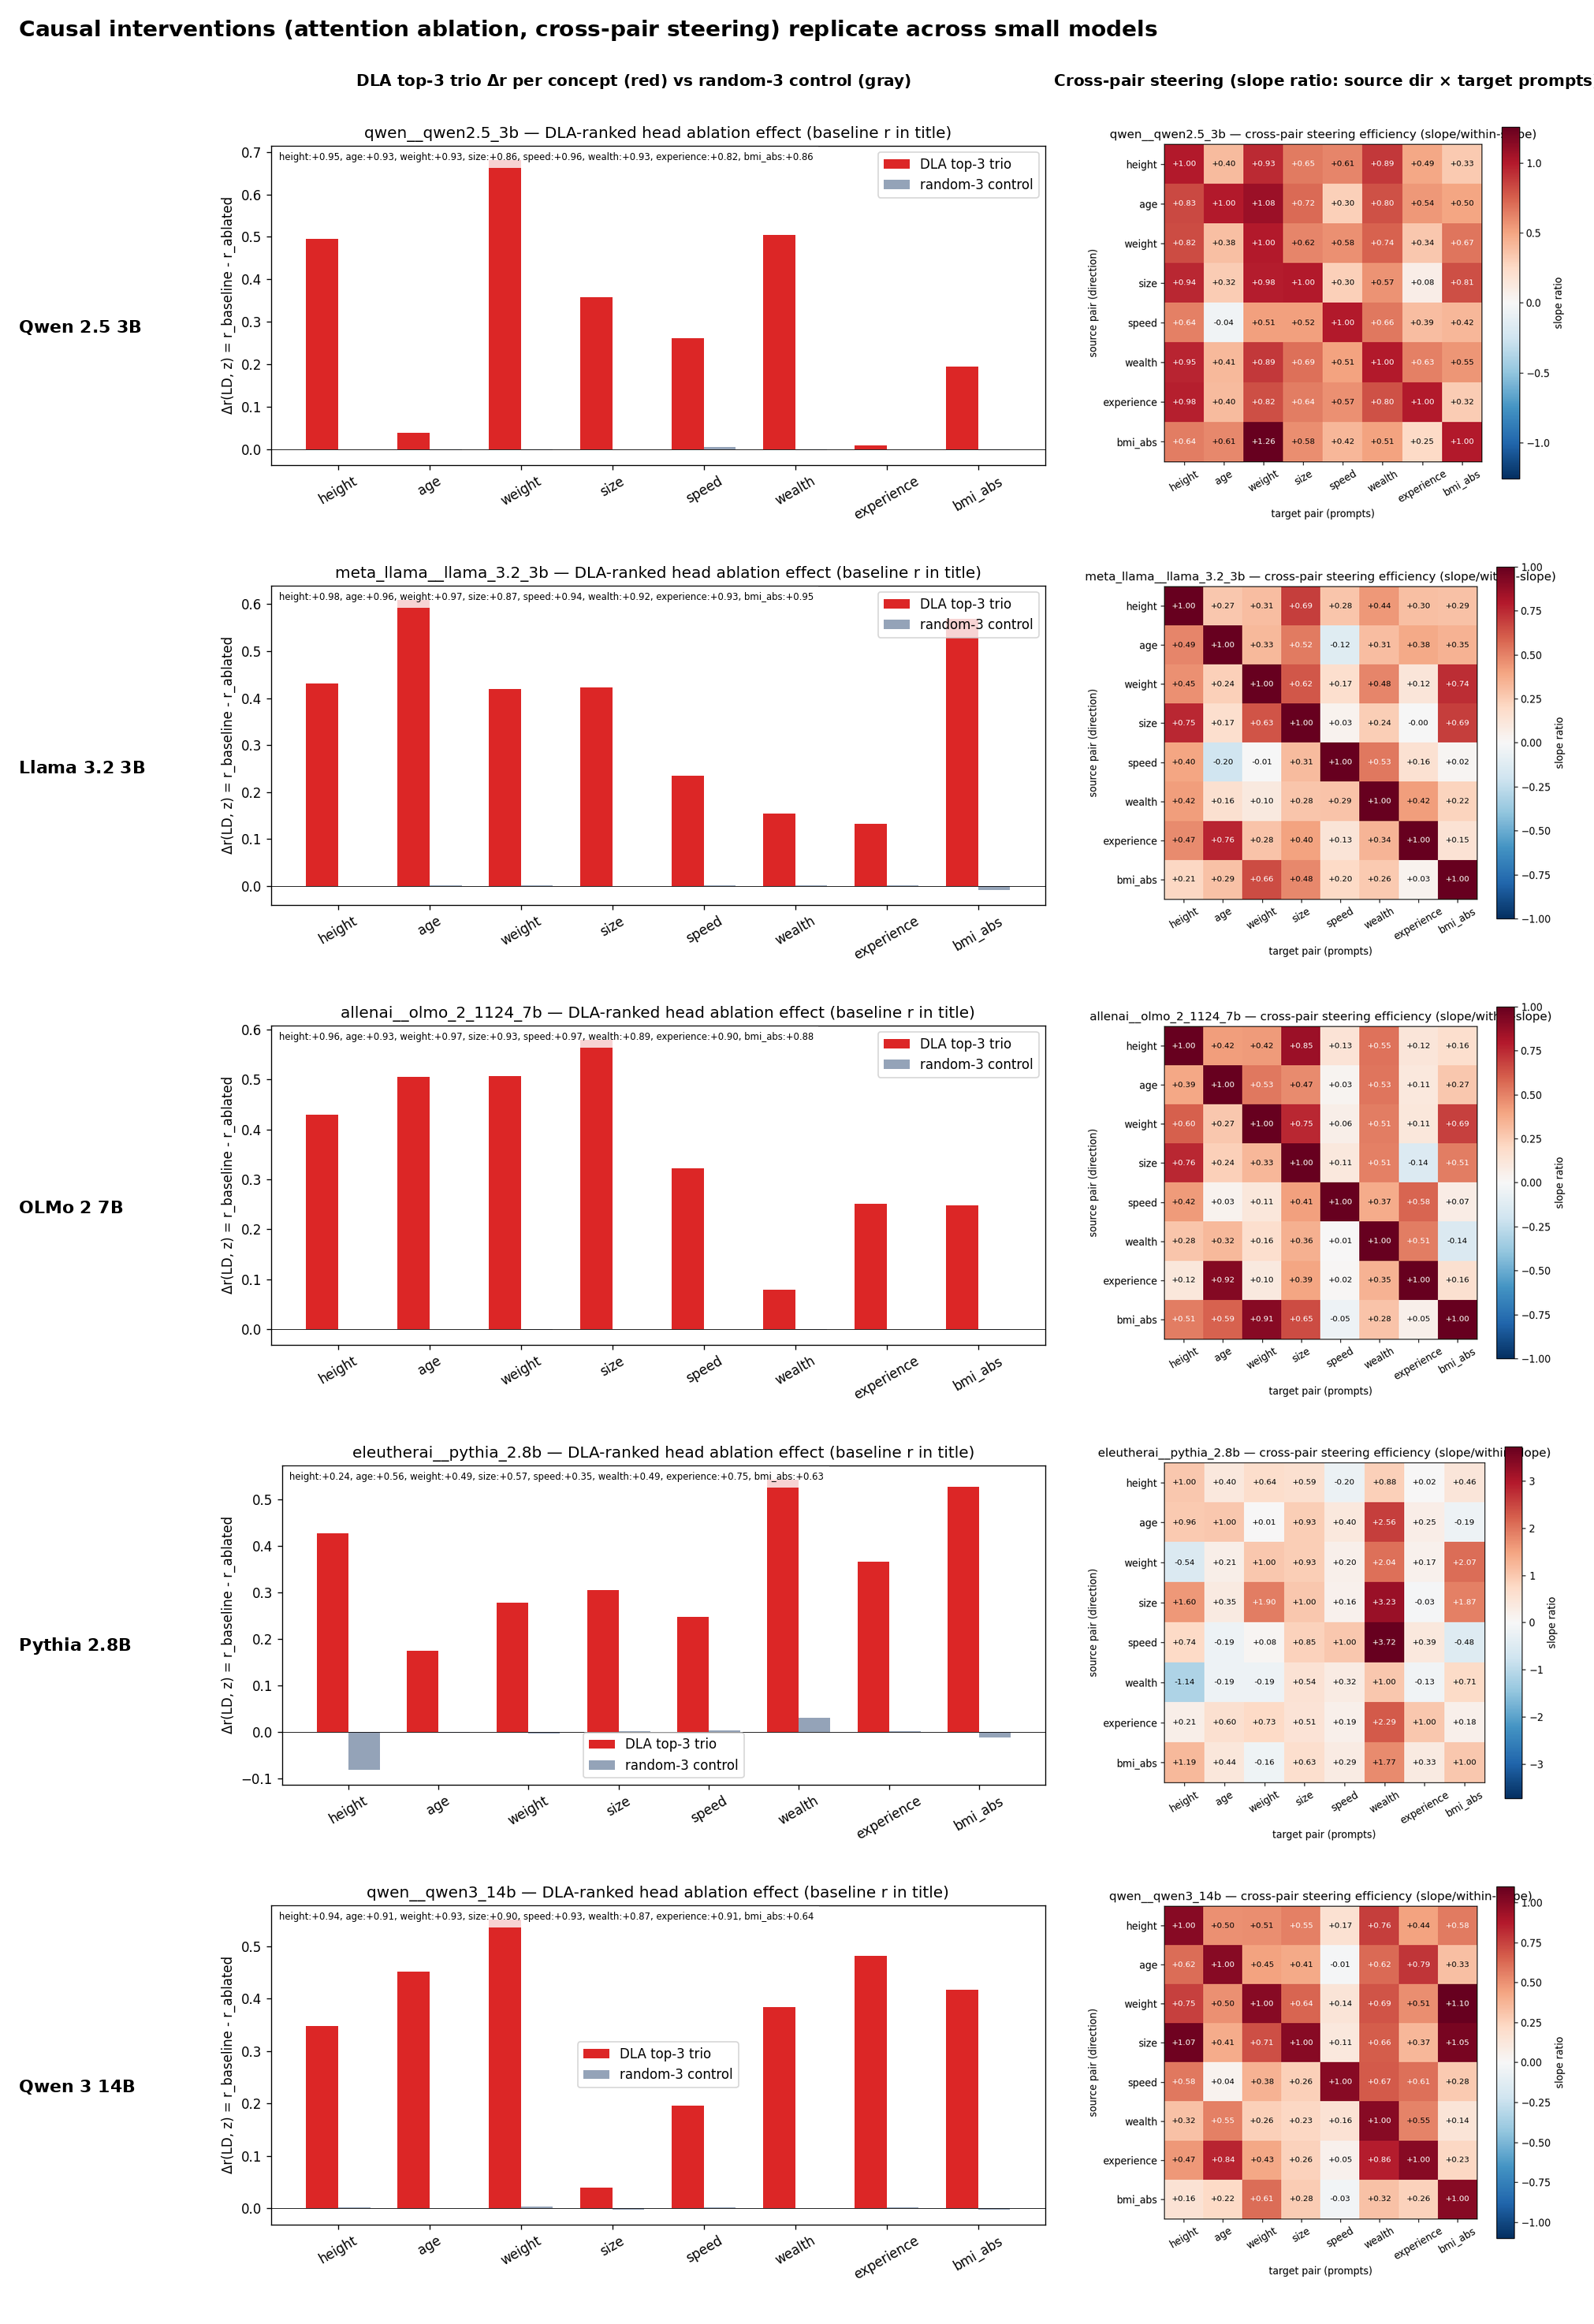
\includegraphics[width=0.8\linewidth]{figures/xmodel_interventions_grid.png}
  \caption{\textbf{Causal interventions replicate across the same five
  models.}
  Rows: Qwen 2.5 3B, Llama 3.2 3B, OLMo 2 7B, Pythia 2.8B, Qwen 3 14B.
  Left column: DLA-ranked top-3 trio interchange ablation
  --- $\Delta r(\mathrm{LD}, z)$ per concept (red) vs same-$N$ random-cell
  control (gray, mostly $\le 0.01$). Trio identification is per-model
  (heads ranked by $\sigma_{\mathrm{DLA}}\cdot|\rho|$ at $k{=}15$ height).
  Right column: cross-pair steering efficiency matrix --- entries are the
  slope ratio when the residual-stream direction estimated on the source
  pair is used to steer prompts from the target pair. Off-diagonal entries
  are predominantly positive across all models except with Pythia 2.8B, indicating that the
  $z$-encoding subspace is shared across concepts (height $\to$ weight,
  weight $\to$ height, etc., transfer with slope ratio $\geq 0.5$ for most
  pairs in every model). Both intervention modes generalize the
  Gemma 2 result.
  % Source: relativity_ablation/scripts/p2v_xmodel_appendix_composites.py;
  %         per-model panels under geometry-of-relativity/figures/v13/.
  }
  \label{fig:xmodel-interventions}
\end{figure*}

\end{document}
